% TEMPLATE for Usenix papers, specifically to meet requirements of
%  USENIX '05
% originally a template for producing IEEE-format articles using LaTeX.
%   written by Matthew Ward, CS Department, Worcester Polytechnic Institute.
% adapted by David Beazley for his excellent SWIG paper in Proceedings,
%   Tcl 96
% turned into a smartass generic template by De Clarke, with thanks to
%   both the above pioneers
% use at your own risk.  Complaints to /dev/null.
% make it two column with no page numbering, default is 10 point

% Munged by Fred Douglis <douglis@research.att.com> 10/97 to separate
% the .sty file from the LaTeX source template, so that people can
% more easily include the .sty file into an existing document.  Also
% changed to more closely follow the style guidelines as represented
% by the Word sample file. 

% Note that since 2010, USENIX does not require endnotes. If you want
% foot of page notes, don't include the endnotes package in the 
% usepackage command, below.

\documentclass[letterpaper,twocolumn,10pt]{article}
\usepackage{usenix,epsfig,endnotes}
\usepackage{setspace} 
\usepackage[utf8]{inputenc}
\usepackage[official]{eurosym}
\usepackage{enumitem}
\usepackage{hyperref}
\usepackage{xcolor}
\usepackage{listings}
\lstset{escapeinside={(*@}{@*)}}

\setcounter{secnumdepth}{3} % default value for 'report' class is "2"

\lstset{
basicstyle=\small\ttfamily,
columns=flexible,
breaklines=true
}

\definecolor{airforceblue}{rgb}{0.20, 0.54, 0.66}

\hypersetup{
    colorlinks=true,
    linkcolor=airforceblue,
    filecolor=magenta,      
    urlcolor=airforceblue,
}

\urlstyle{same}

%%%%%%%%%%%%%%%%%%%%%%%%%%%%%%%%%%%%%%%%%%%%%%%
%BEGIN DOCUMENT
%%%%%%%%%%%%%%%%%%%%%%%%%%%%%%%%%%%%%%%%%%%%%%%
\begin{document}
%%%%%%%%%%%%%%%%%%%%%%%%%%%%%%%%%%
%TITLE PAGE
%%%%%%%%%%%%%%%%%%%%%%%%%%%%%%%%%%
\begin{titlepage}
	\vspace*{2.5cm}
	\Huge
	\begin{flushleft}
	\textbf{ProxyAuth: Continuous Authentication\\ using Bluetooth and Mobile Devices}

	\large
            
	\vspace{3cm}
	\normalsize
	Author:\\ 
	\large \textbf{Ju Hong Kim}

	\vspace{0.5cm}
	\normalsize
	Contributors to the Project\\
	\textbf{Arslan Qamar, Anurag Bist, Sean Coutinho, Ju Hong Kim, Areeb Siddiqui, Daniel Xin Wang}
	
	\vspace{0.5cm}
	Project Link\\
	\large \textbf{\href{https://github.com/zakuArbor/proxyAuth/}{github.com/zakuArbor/proxyAuth/}}
	
            
	\vspace{0.5cm}
	\onehalfspacing
	\begin{singlespace}
	\normalsize Course:\\
	\large \textbf{CSC490 - Security Capstone Design}
	\end{singlespace}
    
    \begin{singlespace}
	\normalsize Instructor:\\
	\large \textbf{Furkan Alaca}
	\end{singlespace}
      
    \begin{singlespace}
	\normalsize Teaching Assistant\\
	\large \textbf{Anthony Tam}
	\end{singlespace}

	\begin{singlespace}
	\normalsize Institution\\
	\large \textbf{University of Toronto Mississauga}
	\end{singlespace}
	
	\vspace{0.75cm}
	\normalsize
	Mississauga, ON, Canada\\
	April 6 2020
	\end{flushleft}
	\vspace{4cm}
            
\end{titlepage}


%don't want date printed

%make title bold and 14 pt font (Latex default is non-bold, 16 pt)

%%%%%%%%%%%%%%%%%%%%%%%%%%%%%%%%%%
%Table of Content
%%%%%%%%%%%%%%%%%%%%%%%%%%%%%%%%%%
\doublespacing
\tableofcontents
\onehalfspacing

%%%%%%%%%%%%%%%%%%%%%%%%%%%%%%%%%%
% Report
%%%%%%%%%%%%%%%%%%%%%%%%%%%%%%%%%%

%%%%%%%%%%%%%%%%%%
% Report Title
%%%%%%%%%%%%%%%%%%
\title{\Large \bf ProxyAuth: Continuous Authentication using Mobile Devices}

\author{
{\rm Ju Hong Kim}\\
\rm \textbf{Email:} juhong.kim@mail.utoronto.ca\\
\rm \textbf{Project Link:} \href{https://github.com/zakuArbor/proxyAuth/}{github.com/zakuArbor/proxyAuth/}
%Your Institution
%\and
%{\rm Second Name}\\
%Second Institution
}
\date{March 7 2020}

\maketitle

% Use the following at camera-ready time to suppress page numbers.
% Comment it out when you first submit the paper for review.
\thispagestyle{empty}

%%%%%%%%%%%%%%%%%%
% ABSTRACT
%%%%%%%%%%%%%%%%%%

\section*{Abstract}
\addcontentsline{toc}{subsection}{\protect\numberline{}Abstract}%
\textbf{Passwords are inherently insecure and easily forgotten. Common passwordless authentications such as iris scanners, fingerprints, and hardware authenticators (i.e. Yubikeys) require additional costs to the user and only perform one-time authentication. One-time authentication relies on users to log out their computers which is not often done due to either inconvenience or clumsiness. This poses a huge security risk as the computer is vulnerable to data theft and tampering with the possibility of malicious software to be installed without the user's notice. Continuous authentication is not widely adopted and requires users to purchase and carry around additional hardware to prevent malicious actors from accessing their machines when users leave their system unlocked.\\
To address this issue, we propose ProxyAuth, an open source continuous authentication that is cheap, convenient, and secure. In ProxyAuth, a user will use their Android phone as a hardware authenticator to authenticate their computer with zero-effort and have their phone continually de-authenticate the system while they are using the computer. The computer will be locked when the user is not nearby the computer. ProxyAuth detects proximity through bandwidth anaylsis between Bluetooth communication of the computer and the phone. The project is still ongoing but is on a great start to replace password-based authentication and never have a computer left unlocked.}

%%%%%%%%%%%%%%%%%%
% INTRODUCTION
%%%%%%%%%%%%%%%%%%
\section{Introduction} 

\subsection{Problem Statement:}
Currently, there is no widely known passwordless authentication method to log into and out of a Linux Desktop Environment using a mobile phone without user interaction. Existing passwordless authentication requires Linux users to have a hardware authentication device such as a Yubikey or a fingerprint scanner. We wish to address the Linux User base who cannot afford to buy additional hardware with the use of a mobile phone as a hardware authenticator instead. Furthermore, these implementations do not offer an auto lockout feature and therefore rely on the user to log out. Users do not often log out of their machines either due to inconvenience or simply forgetting to do so. This can pose a big internal security risk to the company and the individual as the computer would be at risk of having data being stolen or tampered. In addition, attackers could also use this opportunity to install malicious malware to the system to do further damage to the organization. The solution we propose is a cost-effective and convenient method whereby the phone will authenticate the PC via Bluetooth and will continuously de-authenticate the PC when the user is nearby the system.

The goal of the project ProxyAuth is to be an authentication that is convenient, secure, and cheap. To satisfy these goals, these are the key features that ProxyAuth must satisfy:

\begin{singlespace}
\begin{itemize}[noitemsep]
\itemsep0em 
\item Passwordless Authentication
\item Authenticate based on proximity of the phone using Bluetooth
\item Convenient (zero-effort authentication) to increase usability
\item Continuously authenticate/de-authenticate the user when they are within range
\item Lock system once the user is a certain distance away from their PC
\item Prevent Bluetooth amplifier attacks
\end{itemize}
\end{singlespace}

\subsection{Rationale:}
In my personal experience, I often leave my laptop unlocked a lot during my time at IBM as I frequently visit a co-worker, attend meetings, refill my coffee, take a walk, or to go to the bathroom. With my password being over 15 characters, it is a pain to keep authenticating the system each time I leave the system unattended. The project proposal my fellow team members have proposed to me was an excellent solution to my problem. Previously I left my laptop unlocked because I was comfortable with leaving my system unattended with my team in a limited and locked room. However, I may not have the opportunity to work in a secured room when I start working again. Many members of the group had similar issue as me so as a group, this was an issue we wished to address. 

In terms whether or not our skills were well-suited for the project is debatable. The team had members with different amount of skills, experiences, and motivations. I cannot speak for others in the team but my experience and skills were well-suited for the project. ProxyAuth had three main components:
\begin{itemize}[noitemsep]
\item PAM Module
\item Android Application
\item De-authentication Server: A Bluetooth server to continuously send challenge and response to the mobile device  
\end{itemize}

My experience with working on an Android Application with a team of 7 for an Introductory Software Engineering course has given me insight how Android Application Development works. This led me to help other members set up Android Studio and answer any questions they have pertaining to Android. Although I am not familiar with programming Bluetooth nor know what PAM was, I was confident that I could learn quickly. Picking up new skills and learning new things are traits that are expected in the industry. In addition, this project gave me the opportunity to study more about Linux even though it may not be in the Kernel level that I originally wished to work on. I love using Linux and find joy programming in C so working on the PAM module and the Bluetooth server well matched my skills and interests.

\subsection{ProxyAuth}
As of the final sprint (March 29 2020), we have implemented the following:
\begin{enumerate}[noitemsep]
\item A Linux PAM that allows user to authenticate their PC based on the fact that their phone is paired and trusted by the PC (this is done by implementing a Linux Pluggable Authentication Module - PAM)
\item An Android Device that continuously de-authenticate the PC and locks the PC if the phone stops sending messages to the PC
\end{enumerate}

To authenticate the PC, Linux uses PAM which are modules that are used to authenticate a user to any PAM-aware application (in our case, we are trying to authenticate to Gnome Display Manager's login screen, the default Ubuntu login screen). PAM checks through all the devices that are paired with the PC and cross-check the MAC addresses with the list of MAC addresses the user whitelisted. If PAM finds a device that is paired with the PC and is trusted by the user, it authenticates the user and spawns the de-authentication server that will continuously send and receive messages from the paired device that authenticated the PC. If the de-authentication server (a program that runs on the background of the PC) detects that the device trying to communicate with the server is not the device that authenticated with the PC or if the trusted device stops sending messages, the program will lock the PC and terminate itself to prevent any further communication with any devices. The reasons why we choose to authenticate based on Bluetooth or any design decisions can be found under \nameref{Section 5}.

\subsection{Summary of Security Considerations}
When working on the project proposal, we have thought of the following possible attacks:
\begin{itemize}[noitemsep]
\item Spoofing Bluetooth Addresses
\item Bluetooth Amplification Attack
\item Mobile phone being stolen to gain access to the system
\end{itemize}
The project is aimed to be secured so the aim was to prevent Bluetooth spoofing and Bluetooth amplification attack. The only security factor that is not planned to be addressed directly is the loss of the mobile phone (the hardware authenticator). To test whether our project can protect itself from Bluetooth Amplification attack, the department has invested money to acquire two Ubertooth One, an open source 2.4 GHz device that gives us the flexibility to play around with Bluetooth that traditional Bluetooth adapters do not allow. The team has tasked two members to investigate how Ubertooth One works and figure a method to amplify or repeat Bluetooth packets so that we can attack our system. The idea was to amplify Bluetooth packets being sent to and from the PC and the mobile device to gain access to the system when the user is far enough to not realize that someone malicious wants access to his system. Since the packets would be repeated, the communication range of the device and the PC would be extended. Since the team could not successfully use the Ubertooth One to attack the system on time, the team only devised ideas on how to counter this issue. One solution is to check the bandwidth and latency of the Bluetooth packets to determine the distance the mobile phone is from the PC.

To defend against spoofing, the team has been working on ways to encrypt messages between the phone and the PC to determine whether or not the device is who they claim to be. The encryption the team decided to use was AES with GCM to ensure integrity of the message being sent and the authenticity of the message. However, we have yet to test this attack as their was no time to complete the project before the final sprint.

As stated earlier, there is no effective way to counter-measure against the device being stolen. This is not what the project will be focusing on. There are some plans to mediate the issue but those are extra features and will not be worked on during the duration of the development phase of the project.

%%%%%%%%%%%%%%%%%%
% Background and Related Work
%%%%%%%%%%%%%%%%%%

\section{Background and Related Work}  

\subsection{Background}

It is not rare to see workers at a workplace leave their computers on as they take a break. This is a grave concern since the computer is left at a vulnerable position where the loss and tampering of data can occur. Furthermore, the use of stolen or weak passwords is very common. There are many incidents of security breaches in the past decade or two simply due to the use of common passwords. According to the 2017 Verizon Data Breach Investigation Report, "81\% of hacking related breaches leveraged either stolen and/or weak passwords"[1]. This opens up the question of whether or not users have simply given up on security and opted to create and reuse simple passwords for every application they use. As we all know, security breaches cost companies a loss of a lot of resources and reputation.

Passwords are often referred to as the weakest link in security. The use of unique and strong passwords require users to be creative and often lead to forgotten password. In a survey conducted by Forrester, several large organizations allocate over \euro{700 000} annually just for password-related support costs[2]. Passwords are just a pain for both client and security professionals. It is not rare to have employees resetting their password for their work accounts. One survey found 57\% of respondents have to reset their work account which affects productivity[3]. Even if a strong and memorable password were to be chosen, the password is still at risk of being phished. Phising is a common and growing method of attack where about 33\% of breaches were conducted by Social Engineering in 2019 [4]. Another issue with passwords is that they are not resilient to physical observation meaning anyone can watch over the person typing in the password. Due to all of these factors, passwords lack both usability and security benefits that a good authentication method should provide.

It is clear that password-based authentication is not the way IT products and services should adopt. One of the earliest works to make passwords more secure is the use of password managers. Password managers allow users to create strong and complicated passwords that are not easily crackable and have their password managers to remember them. Some examples of password managers are the browsers' built-in encrypted password managers, Dashlane, and LastPass. Password managers are very simple, convenient and scalable to remember passwords for every service one subscribes to. However, password managers are only secure if the master password to the password manager is both secure and memorable. Password managers do not get rid of the entire issue with passwords. This could lead to a big compromise with the attacker knowing all the users' passwords if the master password was to be stolen.

There are three main categories of methods in user authentication[8]. Authenticate based on what you know, what you have, and what you are. There is another category which is where you are which will be explained in detail later.

An example of authenticating users with what you have is Hardware tokens. Hardware tokens such as RSA SecurID aims to replace passwords by having the device cryptographically generate a strong 6-digit code every 60 seconds instead of using a statically user-created password [7]. For the token to work with the authentication module, the device and the module must know the secret "seed" that is unique to the device. This allows the system to authenticate the user based on what they have and to fix the issue with the poor security of passwords due to human cognitive factors. However, some form of password still needs to be written to authenticate the user and acquiring hardware tokens requires the user to buy one.

There has been a lot of movements within the industry to adopt passwordless authentication or multi-factor authentication. It is not uncommon to see many web services to ask users to enter a randomly generated pin code sent to their email or phone on top of their passwords. There also have been moves by many organizations such as Microsoft and Apple to adopt biometric authentication such as fingerprint and iris scanner as an alternative to passwords. Biometric authentication authenticates based on what you are and establishes your identity with your biometric features. Multi-factor authentication has been found to reduce your odds of being compromised by up to 99.9\% according to Microsoft 2018 Security Research [5]. There are many forms and implementation of Multi-factor authentication such as a pin to enter after entering a password, biometrics, SMS, smart cards, and hardware authentication devices such as Yubikeys or tokens. However, the issue with all of these implementations is that they require additional hardware or lacks the user experience. We know from passwords that users simply prefer convenience over security so it is crucial for security professionals to create products that take usability into consideration. 

It is imperative for authentication methods to balance between usability, deployability, and security as proposed in the paper \emph{The Quest to Replace Passwords}. The paper does a great job of proposing a comparative evaluation of different authentication schemes. In their paper, negligible cost is one criterion of deployability that authentication should strive to achieve. Hardware and biometrics authentication such as iris scanner, facial recognition, Yubikey, and fingerprints require the user to invest money to acquire these capabilities. The project we propose ensures no additional cost to the user to gain passwordless authentication. Although ProxyAuth requires users to have an Android Phone and for the PC to have Bluetooth capabilities, we consider this to be a negligible cost to the user. The reason we believe the cost to be negligible is the fact that there are over 5 billion mobile device owners in 2019[9] with about 74\% of the market using Android in December 2019[10]. Iris scanners and fingerprint scanners are not widely adopted in the PC market hence requires additional costs to the users. Furthermore, hardware authenticators such as a Yubikey, which is gaining wide industry adoption, is not convenient to carry around since it is not an object the average consumer carries daily. ProxyAuth proposes users to not carry anything additional than what they normally carry. ProxyAuth provides the "quasi-physically-effortless" usability benefit because the average user carries around their phone daily and so would not be an additional burden. ProxyAuth authenticates users based on what they have and where they are. To authenticate a PC, the user must have their phones with them at all times and be located within the Bluetooth proximity of their device to authenticate. There will be no way to social engineer the user to steal the pin code or a one-time password (OTP) to access the machine. This is an issue with multi-factor authentication because all the attackers need is the password and OTP or pin code which can be all stolen using social engineering. 

We are also trying to offer ProxyAuth as an authentication method that can work side by side with other forms of authentication as well such as password-based authentication, biometrics or other zero-effort authentication. Coupling ProxyAuth with your mobile phone's biometrics and a password to enter to your PC covers all four major methods of authentication: what you know (password), what you have (mobile phone), what you are (fingerprint), and where you are (Bluetooth proximity check) with little to no cost. However, this is not the major focus of the project but is a possible feature to implement in the future. A proximity-based authentication provides ease of use and passwordless authentication. Proximity-based authentication provides all the benefits of passwordless authentication with auto-login and auto-lock features. These features can be extremely useful to those who may need to quickly check the PC for information such as those working in the hospital or the field for surveying. A study in 2005 has found that it is not uncommon for physicians to enter data into the wrong patient's record due to accessing another user's session without knowing[18]. Physicians share the same terminal so when a terminal is found to be unattended, it is not rare for another physician to access the terminal to update a patient's record and forget to log out.

\subsection{Related Works} 
There are a lot of works with creating continuous authentication in the industry. One of the earliest works with continuous authentication is the XYLOC products by Ensure Technologies which uses active RF proximity to detect user's proximity to lock or unlock their machine[12]. Ensure Technologies has been working on proximity-based authentication for an extremely long time introducing XyLoc Secure login for Windows 95. The company requires users to attach a USB device called a lock which will communicate with the key, an authenticator, (which is in the form of a badge or a key chain) that the user will carry around. Just like any proximity-based authentication, the system will lock if the key is a certain configurable distance away from the machine by calculating the strength of the signal between the key and lock. However, the difference between XYLOC and ProxyAuth is how it determines the distance. XYZLOC products require a radio transceiver, the lock, that is attached to the machine that can communicate with the key in 300, 800, or 900MHz radio frequency bands rather than using well-established communication technologies such as Bluetooth which uses 2.4GHz frequency[12]. 2.4GHz and Spread Spectrum technology provides more channels and makes use of more secure communication technologies[11]. ProxyAuth does not require any specialized frequency reader since it relies on built-in Bluetooth adapters and its underlying technology to communicate with the authenticator. Using Bluetooth instead of other radio frequency bands allows us to not worry about dealing with frequency hopping to switch channels to avoid interference from other devices[11]. In addition, the use of an attached USB device clutters one's workspace and is inconvenient to carry around. Traditionally, employees will have their own working area such as a cubicle, where the employee spends most of their time working in their cube. However, with the improving mobile network technology and increasing adoption of laptops, companies are increasing the use of mobile workspace, also referred to as shared workspaces. Carrying additional peripherals to make use of proximity-based authentication is inconvenient. Coupled with the requirement of users to carry around a keycard or a keychain as an authenticator is not a convenient solution at all. ProxyAuth utilizes what existing technologies exist and what users often carry which is a mobile device.

With the increasing interest in smart wearable technologies, there has been work to have wearable devices used for proximity-based authentication. For instance, in WatchOS 3 release, Apple Watch introduced a new feature that unlocks a user's Mac when they are close to their Macbook[13]. However, there does not seem to be any feature within the Apple Watch nor any of their 'Continuity' features that give users an auto-unlock feature when they are not within proximity of their Mac and the auto-lock feature is only offered to Apple Watch users[14]. This may explain why there are $3^{rd}$ party products such as Near Lock Me that provides this feature. Near Lock Me is similar to Apple's unlock feature but the authentication device is the iPhone instead of the Apple Watch and also has the auto-lock feature that ProxyAuth provides[15]. As usual, these features are only offered within the Apple ecosystem and is hardly affordable for the average consumer. Near Lock Me is the closest product that offers the same features as ProxyAuth with the exception that ProxyAuth targets Linux and Android users while Near Lock Me targets the Apple ecosystem. Similar to ProxyAuth, Near Lock Me uses the iPhone as an authenticator. To authenticate the PC, it requires the phone and the PC to be paired and approximates distances using Bluetooth just like ProxyAuth does.

Another related project to ProxyAuth is ZEBRA. ZEBRA is a zero-effort bilateral recurring authentication [17]. The issue ZEBRA is trying to tackle is the prevalent behavior of users leaving their computer terminal unlocked. To authenticate, ZEBRA requires users to wear a bracelet that has a built-in accelerometer, gyroscope, and radio on their dominant wrist which would act as an authenticator. Unlike other related works mentioned that will be mentioned in this paper, ZEBRA takes this approach in a very unique way. ZEBRA compares the wrist movement from the bracelet to the user's input via a keyboard or a mouse to determine the identity of the user. Using the data gathered from the watch such as accelerometer and gyroscope data, the researchers try to correlate it with the input event which seems a very difficult project to implement. The reason why the team did not approach the project towards identifying the user based on the user's behavior is that it goes against the ideals of ProxyAuth. One of the tenants of ProxyAuth is to create continuous authentication without the need for extra hardware or device. Furthermore, the team does not have any background in data science. Therefore, working on a project that requires classifying data and perhaps using machine learning to help improve identifying users is out of the scope.

One neat competitor to ProxyAuth is the use of Glass Wearable Device as an authentication device. Researchers at the Stevens Institute of Technology worked on creating a continuous authentication scheme using glass wearable devices to aid those with disability or provide ease of authentication for those in environments where users need to frequently authenticate and log out such as those working in hospitals[16]. The authentication process works by using a mix of voice and the glasses' vision to authenticate the system. The glasses are meant to be flexible and can have various commands such as "OK glass, authenticate". Using the authenticate phrase would have the system display a QR code in which the user needs to look at to authenticate. The PC would periodically issue authentication challenges which are just QR code that would pop up to the screen. However, wearable glass technologies are still in development and are not widely adopted making the use case for this implementation to not be feasible.

\label{Related Works}

%%%%%%%%%%%%%%%%%%
% Methodology and Design Goals
%%%%%%%%%%%%%%%%%%

\section{Methodology and Design Goals}
\subsection{Methodology}
There are three main components to the project: Android Application, PAM, and a program that continually de-authenticates the PC. The idea is to split the team into two development groups: the Android team and the de-authentication team. We broke the problem for each component to simple manageable parts that can be done in each sprint. The project development cycle we chose is to be agile, making small increments to each component during each iteration of the cycle (i.e. sprint). Whether or not we followed the development cycle is another story. Each feature for each component is supposed to build on top of the previous one so there were not many tasks each member of a team could work on in parallel. The goal was to have all members have the flexibility to either work together or independently to fit each other's schedules. Having an iterative development cycle allows flexibility in changes of project design and switch around user stories depending on what seems to be a higher priority or what can be done within the sprint after taking into consideration other member's schedules. However, we eventually broke some members in the project to the security team. The goal of the security team was to work together in researching the security aspects of the project such as what type of encryption to utilize and how to use the UbertoothOne to attack our project. We dedicated a team to security once the development of each component matured to the point where we had a working implementation that allows a user to authenticate using their mobile device and get locked out if communication with the mobile device and PC ceases.

The overall criteria for the project to be considered a success is to have the ability to authenticate a computer through a user's mobile phone and have the computer locked when the user walks away from the computer.

\textbf{Android Methodology:} The end goal of the Android application is to communicate with the server (the de-authentication program). Therefore, we broke the Android Development into various cycles:
\begin{enumerate}
\item Create a simple Hello World Application - to get an idea of how to create an Android application using Android Studio and how to load the application to their mobile device
\item Find all the devices that has paired with the Android device before
\item Display all the Bluetooth MAC addresses from the previous user story into a list view
\item Have each item in the list lead to a new page in the application (a new activity) with the MAC address to be passed to the new page (an intent)
\item On the new activity, the application should open a new RFCOMM socket (a Bluetooth protocol that provides reliable data stream) to the device we wish to connect to
\item  Once connection is established, create a button that sends a simple string such as "Hello World" to the server
\item Create another button to disconnect from the server
\item Add reading capabilities to the application
\item Create a background service activity which allows the application to continuously  read and write to the server
\item Add encryption and decryption capability to the application \textbf{[NOT COMPLETED]}
\end{enumerate}

\hrulefill

\textbf{PAM Methodology:} The end goal of PAM is to authenticate the computer if the computer can detect the mobile device.
\begin{enumerate}
\item Create a PAM that logs to a file whenever you log in to get an idea of how to work with PAM libraries and how to configure PAM to run your module
\item Create a simple program that scans Bluetooth devices nearby
\item Incorporate Bluetooth scanning program into PAM
\item Allow the computer to be logged in if the developer's phone is detected via Bluetooth scanning
\item Log onto the computer only if the MAC addresses detected is one of the devices that the user trusts (create a file that PAM will read to know which MAC addresses are trusted by the user)
\item Create a program that utilizes D-BUS to get information on what devices are currently paired with the machine
\item Replace authentication to log onto the computer if and only if one of the devices currently paired with the machine is listed under the list of MAC addresses the user trusts. Bluetooth scanning was found to be to slow so we removed this feature.
\item Sanitize all addresses read from the file that contains the list of Bluetooth addresses that the user trusts
\item Fork and execute the de-authentication server once the user is authenticated
\end{enumerate}

\hrulefill

\textbf{De-authentication Server Methodology:} De-authentication server is a background process running on the computer that continuously communicates with the authenticator (mobile device) via Bluetooth to "de-authenticate" the PC. The end goal of the de-authentication server is to continuously issue challenge request to the authenticator and lock the system if the authenticator fails to respond to the challenge.
\begin{enumerate}
\item A Bluetooth server that reads a single input from a connected client
\item Add write capabilities to the server to write back a single message to the client (the Android application)
\item Have the server to continuously interact (read and write) with the client
\item Create lockout feature if the computer fails to get an input from the phone within 10 seconds
\item Only allow the server to connect and communicate with the authenticator that authenticated PAM. If any other device tries to communicate to the server, have the PC locked
\item Have the de-authentication server to kill itself once it detect the user has manually locked out of the machine. This feature was created to prevent conflicts with another instance of de-authentication server that gets spawned each time the user logs in.
\item Add proximity lockout feature by checking the bandwidth of the messages being sent to the server.
\item Add encryption and decryption to the server to create an extra layer of security on top of Bluetooth's encryption \textbf{[Not Completed]}
\end{enumerate}

\subsection{Design Goals}
\large \textbf{Complete Features}:
\normalsize To summarize here are the features that ProxyAuth should provide:

\textbf{Android:}
\begin{itemize}[noitemsep]
\item An application that shows a list of paired MAC addresses to communicate with
\item The list of paired MAC addresses should only display addresses that the user wishes to authenticate to (i.e. should only populate a list of Computer Bluetooth addresses owned by the user) \textbf{Not Completed}
\item Auto pair and communicate with the PC without user's intervention \textbf{Not Completed}
\item A kill switch that simply disconnects with the de-authentication server
\item Add an extra layer of encryption when communicating with the server \textbf{Not Completed}
\end{itemize}

\textbf{PAM:}
\begin{itemize}
\item Login if the device is paired and is trusted by the user
\item Allow customization to PAM to allow multi factor authentication \textbf{Extra  Feature}
\end{itemize}

\textbf{De-authentication Server:}
\begin{itemize}
\item Constantly communicate to the authenticator
\item Auto lockout if the authenticator fails the challenge response request
\item Add an extra layer of encryption when communicating with the Android application \textbf{Not Completed}
\end{itemize}

\label{ssec:num2}

%%%%%%%%%%%%%%%%%%
% Tools and Libraries Used
%%%%%%%%%%%%%%%%%%

\section{Tools and Libraries Used}
\textbf{Hardware}
\begin{itemize}[noitemsep]
\item \textbf{Android Mobile Device}: To act as the authentication device. The minimum Android SDK Version our Authentication Application will support is SDK Ver. 20 which supports the majority of the Android devices currently in use including devices from 2014. The goal of ProxyAuth is to be a cheap alternative compared to other authentication methods and devices. Therefore, we chose to encompass a wide spectrum of Android Devices. There are a few reasons why we choose to work with Android and not alternative operating systems such as iOS and PureOS. Firstly, to develop apps for iOS, you need Xcode which only runs on macOS. This is a big issue as this would require members to purchase Macbooks as only one person in the group runs MacOS. Other alternatives such as Blackberry 10 and PureOS are not valid choices either. Alternative operating systems are not widely adopted which would defeat the purpose of the project. Android OS was ideal because it is the current dominant OS in the market by adoption and is open source with a vibrant community in which we could consult with.

\item \textbf{Linux Computer:} The system we wish to authenticate to. The computer must have Bluetooth support and enabled. Bluetooth is essentially equipped on every Computer being sold in the market for a long time so this should not pose an issue on the user. Development and testing were done on Ubuntu 18.04 LTS since we initially wanted to work on the lab machines. However, due to the lack of permissions on the lab machines, we have opted to use our laptops to test our PAM module.

\item \textbf{Bluetooth Adapters:} Much to our surprise, the lab machines do not have Bluetooth Adapters. However, since there was no way we would get approval to develop our PAM module on the lab machines, that was not an issue. But when developing and testing the project, members initially used a virtual machine which required an external Bluetooth adapter for the virtual machine to have Bluetooth capabilities.

\item \textbf{Ubertooth One:} Ubertooth One is an open source 2.4 GHz wireless development platform that is suitable for Bluetooth experiment. Reading up on a few experiments others have done using Ubertooth One, we thought we could use these neat devices to attack our program by using a repeater attack to extend the signal of the Bluetooth signal. Due to the limitations most Bluetooth adapters have and the fact that Bluetooth technology is not a very open technology, Ubertooth One was the ideal candidate since it was an open source device that will give us enough control of the hardware. Refer to \textbf{\nameref{Section 6.3}} on what our progress was with the device.
\end{itemize} 

\hrulefill

\textbf{Software}
\begin{itemize}[noitemsep]
\item \textbf{Android Studio:} Required to work on the Android Application as it comes with the required tools, plugins, API. Android Studio is also the IDE of choice by the Android Development community so there are a lot of forums and documentation. Using other IDE such as IntelliJ or Eclipse requires more set up to do which would have hindered our progress with the Project.
\item \textbf{GNOME Desktop Environment:} ProxyAuth will only support any Linux systems using GNOME as their desktop environment due to the implementation of PAM and the de-authentication server using GNOME's D-Bus libraries.

\item \textbf{Ubuntu 18.04 LTS and Ubuntu 19.04:} The distribution of choice was Ubuntu since most members are familiar with Ubuntu. The lab machines all use Ubuntu 18.04 LTS so we initially thought we could develop on those machines. Our choice for Ubuntu propelled our implementation of ProxyAuth to support GNOME environment only

\item \textbf{C Compiler - gcc ver. 7.4:} We chose to use gcc simply because it was the compiler that was installed on the lab machines. Using different versions of gcc such as gcc ver. 9.2.1 should and did not matter during development as long as the program can compile using C11(201112L). To find the gcc version, run the following command: \emph{gcc -dM -E - $<$ /dev/null $|$ grep $\_\_$STDC$\_$VERSION$\_\_$}
\item \textbf{Linux PAM Module:} By changing the configuration of GDM (GNOME Display Manager) password configuration file, we can allow users to authenticate their system using our PAM Module. PAM is what Linux uses for authentication.

\item \textbf{Virtual Box:} Any virtual machine application such as VMWare is acceptable. There were no restrictions on what virtual machine the team used. Observing the entire team, most have adopted to use Virtual Box. Most members of the team did not have Linux installed on their machine nor were willing to install Linux on their machines initially. Therefore, some have opted to use a virtual machine to run Ubuntu. However, later in the development stage of the project, the use of virtual machines was dropped. See section \textbf{\nameref{Section 6.3}} for more details as to why we dropped the practice.

\item \textbf{D-Feet:} A neat program to debug D-Bus messages. D-Feet is used to visualize what objects are returned from certain D-Bus calls during development.
\end{itemize}

\hrulefill

\textbf{Programming Language and Scripts:}
\begin{itemize}[noitemsep]
\item \textbf{C:} C was the language of choice since Linux, PAM and a lot of libraries we used were implemented in C. The standard language to develop PAM Modules is C. Although there are small movements to write Linux and C programs in Rust, a programming language that is garnering support within the community due to speed and memory safety performance, it still lacks the years of documentation that C has. C is also the standard language to be taught at the University of Toronto so members of the ProxyAuth group should be more comfortable with the language as opposed to C++ which is very similar to C. Since we were not working on object-oriented programming paradigm, there was no need to work with C++.

However, there was always the option to write most of PAM code in other languages and have our PAM execute our code in another language such as Python. Polyglot programming may allow us to complete tasks much faster by writing components of the code in languages we are most comfortable with but this is just simply a lazy and messy implementation when working on projects that are meant to be coded in languages that are traditionally written in "lower" level languages.

The de-authentication server was also written in C. Although the de-authentication server could have been written in Python, I opted to write the program in C simply because we already invested a lot of time learning the Bluetooth Stack in C. Although this may not be a valid reason, as the main developer for PAM and a major contributor for the de-authentication server, I dislike Python and wanted to practice my C skills so I opted to write the program in C. There are a few reasons to not choose Python for the de-authentication server such as performance of Python and the fact that Python does not have Bluetooth support as part of the standard distribution. PyBluez is simply a Python extension module written in C that uses the official Bluetooth stack from C to gain Bluetooth support. The de-authentication server will be constantly be running so those who use laptops may notice a slight battery life drop compared to running the program in C. This may be negligible as we envision the program to be lightweight for both the mobile phone and computer. See section \textbf{\nameref{Section 6.3}} for more details.

\item \textbf{Kotlin:} Several languages that can be used when developing Android Applications are Java, Kotlin, Flutter or React Native. Although all members are familiar with Java, the Android team opted to use Kotlin rather than Java simply because Kotlin code was more concise. There are other benefits such as having some modern features in the language and its built-in null safety. In addition, Kotlin is more Android focus with a lot of support from the Android Development community to adopt the language as the primary language for Android Development.
\item \textbf{Perl:} Perl was the scripting language of choice. Bash while being an excellent alternative, I am more familiar with Perl. Perl is a very versatile language that is installed in virtually every Linux system so there is no grave concern for users to install Perl. However, I would agree using Perl to install dependencies for PAM and de-authentication server is overkill and can simply be implemented in Bash.
\end{itemize}

\hrulefill

\textbf{Collaboration/Project Management Tools:}
\begin{itemize}[noitemsep]
\item \textbf{Slack:} Slack was the communication tool of choice. Slack is a team collaboration messaging platform that allows us to create channels based on the components of the project. For instance, the Android Development Team Channel will be a channel to discuss any topics, issues, or advancement in the Android Application. Slack also offers integrating apps to enhance our productivity. After noticing how members were not checking Github for updates regularly, I have integrated Github to Slack so that everyone can be notified of any changes in issues, commits, and pull requests.
\item \textbf{Github:} Github is a platform that hosts our code base for the project. Using git as our version control, we can allow multiple collaborators to work on the project at the same time and make use of all the neat features Github offers. Github is a well-polished software platform and is the platform all members of our group are experienced with. Familiarity with the platform is the main reason we chose to use Github over other competitors such as Gitlabs. Github has a lot of features that we took advantage of such as creating issues, creating pull requests at ease, and the Github Issue Board. Github issue board (essentially a Kanban Board) allows us to organize user stories and be able to visualize what user stories are being worked on and what user stories need to be worked on during the sprint. What is neat about Github issues is that you can link issues to pull requests and to milestones. So whenever a pull request gets approved, all the issues on our Kanban board would be moved to the list of tasks that are Completed. 
\end{itemize}

\hrulefill

\textbf{Additional Software Package}
\begin{itemize}[noitemsep]
\item \textbf{Bluez:} Bluez is the package that provides Bluetooth protocol stack. Bluez is the official Linux Bluetooth Stack kernel module and is included in the Linux kernel since Linux 2.6. But to work with Bluetooth in the user space, Bluez User Space package must be installed.
\item \textbf{GLib}: a bundle of 3 low-level system libraries written in C. We required the use of GLib to use the GIO (GNOME Input Output) stack for D-Bus calls. We opted to use \textbf{GDBUS}, GNOME's implementation of D-Bus is based on GIO streams simply because it seemed to be much simpler to work with D-Bus rather than working on other implementations of D-Bus such as libdbus, QtDBus, and sd-bus. D-Bus calls were needed for the project to determine whether a mobile device was paired with the system and to check if the user's session was locked.

\item \textbf{PAM(3)}: is a set of libraries that handles the authentication tasks of applications on the system. Linux uses PAM (Pluggable Authentication Module) modules to handle authentications of various applications such as GNOME Display Manager which is the default login screen for Ubuntu. The libraries must be installed on the machine to work on PAM.
\end{itemize}

\hrulefill

\textbf{Tools We Would have Used -}
Here is a list of tools that could and would have been used if the project has progressed further:
\begin{itemize}[noitemsep]
\item \textbf{Apache 2:} The HTTP Server to host a website where users can notify that they have lost their device. This would be useful to have the device being blacklisted from authenticating any of the users' devices (Extra Feature)
\item \textbf{Router:} To run the wifi network to verify that the devices can only authenticate if they are not only communicating with the Bluetooth server but also on the same network.
\end{itemize}
\label{Section 4}

%%%%%%%%%%%%%%%%%%
% Project Description
%%%%%%%%%%%%%%%%%%
\section{Project Description}
\label{Section 5}

\subsection{System Overview:}
There are three components to ProxyAuth:
\begin{itemize}[noitemsep]
\item Android Application under \textbf{proxyAuth$/$android}
\item Linux PAM module under \textbf{proxyAuth/pam/src/pam\_proxy.c}
\item De-authentication Server under \textbf{proxyAuth/pam/src/deauth.c}

\end{itemize}
This section will describe our approach for proximity and continuous authentication.

A. \textbf{One-time Authentication}\\
Initially authenticating with a system using Proxy comprises of the following steps below:
\begin{enumerate}[noitemsep]
\item Turn Bluetooth on for both the Android phone and the Linux PC
\item Pair the devices to each other
\item Lock the PC
\item By waking up the Linux PC, ProxyAuth PAM should be able to detect the authenticator is paired with the machine and authenticate the user
\item Before ProxyAuth PAM terminates, PAM will fork a new process and execute the de-authentication server
\end{enumerate}

B. \textbf{Continuous Authentication}\\
After the user is authenticated, the de-authentication server will run in the background. Here are the steps of how the current implementation of continuous authentication works:
\begin{enumerate}[noitemsep]
\item De-authentication server is spawned and is given the Bluetooth address of the device that authenticated the user's desktop
\item On the Android device, the user is to open the Android application and select the PC the user wishes to de-authenticate
\item De-authentication server will receive a connection request from the Android device. The server will be given a MAC address when spawned. This MAC address allows the server to know what MAC address authenticated PAM. The server will compare this address to the address of the device that is trying to connect to the server to check if the device is trusted, paired, and is the address that authenticated the desktop
\begin{itemize}
\item If the device is trusted by the user and is paired with the desktop, then the server will communicate with the Android device
\item If the device is either not trusted by the user or not paired with the desktop currently, the server will lock the desktop
\end{itemize}
\item Once the Android application is connected to the server, the application will send messages to the server to indicate it's identity and that the application is still alive and read messages from the server
\item The server will read and write back to the application and it will do the following behaviors:
\begin{itemize}
\item If the server does not receive a message from the server within 10 seconds, the server will lock the desktop
\item If the server detects the rate in which the application is sending is below a certain threshold, the server will lock the system because the authenticator is too far from the desktop
\item If the user manually locks the system, the server will close its communication with the server and terminate
\end{itemize}
\end{enumerate}


\subsection{Prerequisite For Both End Users and Developers}
There are some steps both end users and developers need in their system before using or starting to develop ProxyAuth. 

\textbf{Hardware Requirements:}
\begin{itemize}[noitemsep]
\item A Linux system that uses GNOME as their desktop environment with a Bluetooth adapter
\item A smartphone running Android
\end{itemize}


The following packages must be installed on a Linux system that uses GNOME as their desktop environment:

\begin{itemize}[noitemsep]
\item \textbf{libpam0g-dev} - needed to compile and work with PAM
\item \textbf{libglib2.0-dev} - needed to work with GNOME's D-Bus calls
\item \textbf{bluez} - needed to work with Bluetooth on Desktop
\item \textbf{libbluetooth-dev} - needed to work with Bluetooth on Desktop as well
\end{itemize}
These dependencies can simply be installed on any Debian system by running \textbf{sudo make install} under \textbf{proxyAuth/pam} assuming you have cloned the project.\\
\textbf{Note:} ProxyAuth currently only supports Linux with GNOME and Android devices only. Refer to \nameref{Section 4} for more details what software and hardware are needed for the project or for more information of what each library and dependencies are for.

After installing all the dependencies for the project, create the directory \textbf{/lib/security} if it does not exist. \textbf{/lib/security} is where any non-default PAM modules are located (and is also where ProxyAuth PAM module will be residing).

The next step is to change PAM GDM Password configuration. Add the following lines to the top of \textbf{/etc/pam.d/gdm-password} with \emph{sudo} or as \emph{root}:
{\small
\begin{verbatim}
#proxyAuth
auth sufficient pam_proxy.so
auth required pam_warn.so
\end{verbatim}
}

This is needed to indicate that we wish to allow desktop login using our PAM module.

\textbf{To add a trusted device:}
\begin{itemize}[noitemsep]
\item Create the directory if it does not exist: \textbf{/etc/proxy\_auth/}
\begin{itemize}[noitemsep]
\item This is where all the user's MAC addresses are stored and where the de-authentication server will be located
\end{itemize}
\item create a file that is named after the username of the user
\item add to the file the MAC address of the authenticator\\
Steps 2 and 3 can be done using the following command: \textbf{sudo echo \emph{bluetooth\_address} $>>$ /etc/proxy\_auth/\$USER}
\end{itemize}

\textbf{Running Bluetooth Server:}
There are issues with the \textbf{sdptool} in Bluez 5 when trying to run a Bluetooth server. Therefore there are some steps that needs to be added before running ProxyAuth:
\begin{enumerate}[noitemsep]
\item Open the Bluetooth configuration that your Bluetooth service loads for editing. To find out which configuration file your system loads, run the following command: \textbf{sudo systemctl status bluetooth}\\
The following output should be something similar to the output below:
{\small
\begin{lstlisting}
$ sudo systemctl status bluetooth
 bluetooth.service - Bluetooth service
   Loaded: loaded (/lib/systemd/system/bluetooth.service; enabled; vendor preset
   Active: active (running) since Wed 2020-04-01 00:34:23 EDT; 7s ago
     Docs: man:bluetoothd(8)
 Main PID: 8903 (bluetoothd)
   Status: "Running"
    Tasks: 1 (limit: 4915)
   Memory: 1.1M
   CGroup: /system.slice/bluetooth.service
           8903 /usr/lib/bluetooth/bluetoothd
\end{lstlisting}
}

The Bluetooth configuration file is \textbf{/lib/systemd/system/bluetooth.service} according to the output above. Some systems may use \textbf{/etc/systemd/system/dbus-org.bluez.service} instead depending on the distribution and version the system is running on.

\item Change the following line: \textbf{ExecStart=/usr/lib/bluetooth/bluetoothd} to \textbf{ExecStart=/usr/lib/bluetooth/bluetoothd --compat}

\item Add the following line to the file: \textbf{ExecStartPost=/bin/chmod 777 /var/run/sdp}\\
The permissions of /var/run/sdp changes on each reboot which is why the above line is needed to update the permission each time the system boots up. This is to avoid segmentation fault when running sdp tools which is broken in Bluez 5. Not sure when Bluez team will fix this issue.

\item Restart bluetooth with the following commands:
{\small
\begin{lstlisting}
sudo systemctl daemon-reload
sudo systemctl restart bluetooth
\end{lstlisting}
}
\end{enumerate}

Now that all the dependencies, directories, and files have been created or modified, the user and developer can now start using the project.
\label{prerequisite}

\subsection{PAM Implementation}
Linux PAM (Pluggable Authentication Module) enables the local system administrator to choose how applications authenticate users[19]. A PAM module takes the form of a dynamically loadable object file (with the extension \%.so). Meaning PAM modules are dynamically linked at runtime whenever a specific application relies on PAM API for authentication. PAM modules allow developers to develop applications separate from the authentication scheme. Refer to \textbf{proxyAuth/Makefile} to see how to compile PAM modules since it is different from compiling code to be an executable. The file is also a good reference to know how to compile code using Bluez and GLib since some libraries require more than just adding a library flag to compile.

For the project, we want to edit the policy of how \textbf{gdm-password} authenticates users. In the subsection above, we modified \textbf{gdm-password} because the program that handles graphical user interface logins on machines using GNOME relies on \textbf{gdm-password}. We have added the following rule to \textbf{gdm-password}:
{\small
\begin{lstlisting}
auth sufficient pam_proxy.so
\end{lstlisting}
}
The \emph{auth} module group deals with authenticating the user. \emph{sufficient} control flag allows us to have PAM recognize a success with the module we created, \textbf{pam\_proxy}, to be all that PAM needs to allow access to the user if our module returns a success.

Once PAM configuration has been finished, the actual PAM module development starts. When GDM loads \textbf{pam\_proxy.so} to authenticate the user, the service function \textbf{\emph{pam\_sm\_authenticate}} will be called which can be found under \textbf{proxyAuth/pam/src/pam\_proxy.c}. To authenticate the user, \textbf{\emph{pam\_sm\_authenticate}} must return \textbf{PAM\_SUCCESS}. In \textbf{pam\_proxy.c}, a \textbf{PAM\_SUCCESS} will only be returned if a trusted Bluetooth device is paired to the system. This is done via calling a function named \textbf{\emph{bluetooth\_login}} which is defined in the file \textbf{pam\_bt\_trust.h}. There are three main steps \textbf{\emph{bluetooth\_login}} does to find whether or not a device is allowed to authenticate the device:
\begin{enumerate}[noitemsep]
\item Get a list of MAC addresses that are currently paired to the system via \textbf{\emph{get\_paired\_devices}} function call
\item Get a list of MAC addresses the users trust via the function call \textbf{\emph{find\_trusted\_devices}}
\item The function \textbf{\emph{find\_trusted\_paired\_device}} takes in the lists created from \textbf{\emph{get\_paired\_devices}} and \textbf{\emph{find\_trusted\_devices}} and returns a MAC address of the first MAC address that exists in both lists or NULL if there is no such device.
\end{enumerate}

\subsubsection{Get List of Paired Devices}
To get a list of devices that are currently paired to the system in \textbf{\emph{get\_paired\_devices}}, a D-Bus call must be made. D-Bus is a message bus system that allows applications to talk to one another. We will be using GDBus, an implementation of D-Bus based on GIO streams used in GNOME applications. The D-Bus call is done by the function \textbf{\emph{get\_paired\_devices}} defined under \textbf{pam\_bt\_pair.h}. The file \textbf{pam\_bt\_pair.h} deals with any function related to gathering the list of paired devices. The function will make the following call to D-Bus to get a list of objects from Bluez: 
{\small
\begin{lstlisting}
DBUS_NAME: "org.bluez"
OBJECT_PATH: "/"
INTERFACE: "org.freedesktop.DBus.ObjectManager"
METHOD: "GetManagedObjects"
\end{lstlisting}
}
The D-Bus call will not return you a list of Bluetooth devices that are currently paired with the device but a list of Bluetooth devices that the system detects. Therefore, the object returned by the call will need to be parsed which is done by the function \textbf{\emph{process\_dbus\_bt\_list}}. Essentially, the function will parse through every device object and check if the property \textbf{Connected} is True. The property \textbf{Paired} is not of great importance since the property is set to True if the device has been paired with the system before but does not tell us anything if the device is currently paired to the system. A sample device object is shown below for reference:
{\small
\begin{lstlisting} 
{'Adapter': '/org/bluez/hci0',
 'Address': '20:DA:22:DE:0F:68',
 'AddressType': 'public',
 'Alias': 'kimju10',
 'Blocked': False,
 'Class': 5898764,
 'Connected': True,
 'Icon': 'phone',
 'LegacyPairing': False,
 'Modalias': 'bluetooth:v010Fp107Ed1436',
 'Name': 'kimju10',
 'Paired': True,
 ...
}
\end{lstlisting}
}
\subsubsection{List of Devices Trusted by the User}
The function \textbf{\emph{find\_trusted\_devices}} is responsible for returning a list of Bluetooth addresses that are trusted by the user. In our implementation, each user in the system will have a file under \textbf{/etc/proxy\_auth/\emph{username}} which represents a list of Bluetooth MAC addresses the user trusts to authenticate their system separated by newlines.
When working with PAM, \textbf{\emph{pam\_get\_user()}} can be called to get the username of the user trying to be authenticated. Using the username, the function will read from the list of Bluetooth MAC addresses the user trusts from the file under \textbf{/etc/proxy/proxy\_auth/\emph{username}} and place them to an array. When reading from a file, it is best to not trust the file so sanitization is done when parsing through the list of addresses from the file to check if the address is a valid Bluetooth address.

\subsubsection{Executing the De-authentication Server}
If \textbf{\emph{find\_trusted\_paired\_device}} finds a Bluetooth address that appears in both the list of trusted devices and in the list of paired device, it will return the address to \textbf{\emph{bluetooth\_login}}. Since there exists a trusted device that is paired to the system, \textbf{\emph{pam\_sm\_authenticate}} will call \textbf{\emph{exec\_deauth}} defined in the file \textbf{pam\_post\_auth.h}. If there does not exist a paired device that is trusted, then \textbf{\emph{pam\_sm\_authenticate}} will return \textbf{PAM\_AUTH\_ERR} to indicate a failure to authenticate the user and will not spawn a de-authentication server.

\textbf{\emph{exec\_deauth}} responsibility is to fork and exec the de-authentication server which is located in \textbf{/etc/proxy\_auth/deauth} which will communicate with the Android device. To create a new process in C, \textbf{\emph{exec}} must be called. However, \textbf{\emph{exec}} replaces the current process so a fork must be called to avoid replacing the current process. The de-authentication server takes in one mandatory parameter which is the MAC address of the device that authenticated PAM. It is not clear to Kim whether or not a process spawned in the PAM module runs as root but to prevent unneeded privilege escalation issues and to have the de-authentication server auto-lock feature to work, the \emph{euid} of the \textbf{deauth} will be set to the user instead of root. Once the server is executed in a child process, \textbf{\emph{pam\_sm\_authenticate}} will return \textbf{PAM$\_$SUCCESS} to indicate GDM that the user is authenticated and therefore give access to the user their account.

\subsection{De-authentication Program}
The role of the de-authentication server is to communicate with the authenticator and lock the system once it detects an issue with the authenticator such as not receiving input from the authenticator or detects that the authenticator is far from the system (PC). The server is spawned by our PAM module and takes in a single parameter which is the MAC address of the device that authenticated PAM. The source code can be found under \textbf{proxyAuth/pam/src/deauth.c}. 

\subsubsection{Checking Deauth's Argument}
Before starting the Bluetooth server, there are a few things \textbf{deauth} does. Firstly, \textbf{deauth} checks if the given parameter is a valid Bluetooth address by calling the function \textbf{\emph{check\_arg}}. In addition, \textbf{deauth} also verifies that the given Bluetooth address is currently paired and trusted by the user by calling \textbf{\emph{is\_trusted\_client}}. If any of the two functions return False, the program will lock the system. The given Bluetooth address is needed to know which device to communicate with. It is dangerous to accept a connection from a random device.

\subsubsection{Bluetooth Overview} 
When working with Bluetooth, it is helpful to understand some fundamentals about Bluetooth, especially if you are trying to understand what is going on in the function \textbf{\emph{init\_server}} in \textbf{deauth.c}. Bluetooth is a short-range wireless technology (operating at 2.4GHz) with a maximum range between 10-100 meters depending on the Bluetooth class the device has[20]. Typical mobile phones have only Bluetooth class 2 or class 3 which have a range of 10m or less which is perfect for our use case. Since we want the program \textbf{deauth} to act as a server, we need to advertise \textbf{deauth} as a service to all the devices around the PC. The PC will act as a Service Discovery Protocol server which will advertise all services registered to the SDP server. This allows our phone to be aware of the \textbf{deauth} service and connect to it.

Special thanks to \textbf{Albert Huang} for his documentation on programming Bluetooth in Linux. Without his work, working with Bluetooth would have been an almost impossible task.

The function \textbf{\emph{init\_server}} binds the Bluetooth socket to some port and register the service by calling \textbf{\emph{register\_service}}. \textbf{\emph{register\_service}} is where all the set-up for the Bluetooth server occurs and is quite difficult to understand without knowing anything about how Bluetooth works. I have broken down the Bluetooth server to the following functions and will briefly go over in a high level what is going on in each function:
{\small
\begin{lstlisting}
set_service
set_bluetooth_service_info
set_browsable
set_l2cap_info
register_rfcomm_sock
register_service
\end{lstlisting}

Refer to \textbf{figure 1} to see an overview of some definitions that may serve useful in understanding some terminologies that will be used in this section. It is useful to also refer to \textbf{figure 2} to see what attributes are in a service record. Both \textbf{figure 1} and \textbf{figure 2} are located at the end of this \textbf{section 5.4.2}.

\hrulefill

\textbf{\emph{set\_service}}\\
This function is responsible for setting a UUID to identify the \textbf{deauth} as a service. Each service is identified by a UUID which is a 128 bits long but is often shortened to 16 or 32 bits. Since our application is not close to any well-known services we'll be generating our own custom 128 bit UUID for the general service ID. The function will also generate another UUID to register the service class id of the service. \textbf{Service Class ID} identifies the type of service our service is. Since the service we are creating is an instance of the \textbf{Serial Port Service Class}, we set the service to be \textbf{SERIAL\_PORT\_SVCLASS\_ID}. Take note that all information pertaining to the service is stored in a service record. Refer to \textbf{figure 2} at the end of \textbf{section 5.4.2} to see a diagram of what attributes are stored in a typical service record

\hrulefill

\textbf{\emph{set\_bluetooth\_service\_info}}\\
This function is responsible for setting the profile of the service we are trying to create. Bluetooth profiles are additional protocols that help define what kind of data the service is transmitting[22]. The profile the program will use is \textbf{Serial Port Profile (SPP)} which are great at sending a lot of data between the PC and the authenticator.

\hrulefill

\textbf{\emph{set\_browsable}}\\
This function is responsible to set our service record to be publicly browsable. Note: We have not yet registered our service record to the SDP server so the service is not yet advertised by the SDP server.

\hrulefill

\textbf{\emph{set\_l2cap\_info}}\\
This function creates a UUID for L2CAP and to indicate our service will be using L2CAP protocol. When our service is discoverable with SDP, there are various ways to access our service. We will be using L2CAP protocol (Logical Link Control and Adaptation Protocol) to handle communication between the server and client[23].

\hrulefill

\textbf{\emph{register\_rfcomm\_sock}}\\
The function is responsible to register the RFCOMM channel for RFCOMM sockets. RFCOMM (Radio Frequency Communication) is a protocol built on top of L2CAP protocol [28]. RFCOMM provides a simple reliable data transfer similar to TCP.

\hrulefill

After \textbf{\emph{register\_service}} calls all the above functions, all that is left is to register the service to our local SDP server. Before registering our service, we should give some metadata about our service such as the service name, provider and description which is done by using Bluez's function \textbf{\emph{sdp\_set\_info\_attr}}.

To register the service to the local SDP server, we need to first connect to the SDP server using Bluez function \textbf{\emph{sdp\_connect}}. The function to register our service is \textbf{\emph{sdp\_record\_register}}.

To summarize, here is the flow of how to set up a Bluetooth server taken from \textbf{Albert Huang's} book \textbf{\emph{Bluetooth Essentials for Programmers}}[25]:
{\small
\begin{lstlisting}// set the general service ID
// set the service class
// set the Bluetooth profile information
// make the service record publicly browsable
// set l2cap information
// register the RFCOMM channel for RFCOMM sockets
// set the name, provider, and description
// connect to the local SDP server and register the service record
\end{lstlisting}

\hrulefill

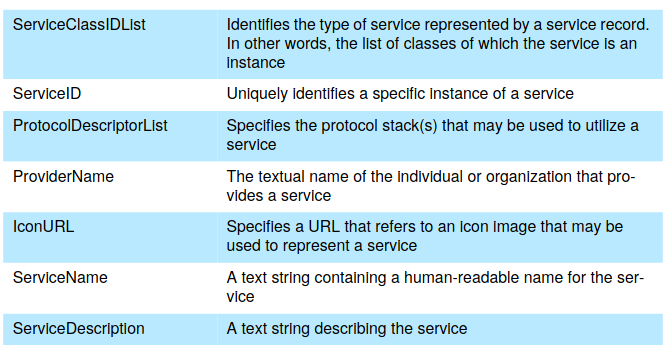
\includegraphics[scale=0.3]{bluetooth-definitions.png}
\small \textbf{Figure 1:} A list of common definitions taken from \textbf{Bluetooth Specification Version 1.0 B}[24]

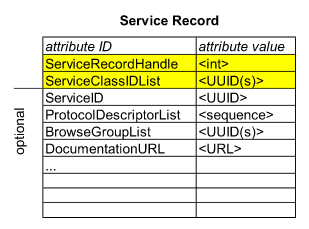
\includegraphics[scale=0.5]{bluetooth-service.png}\\
\small \textbf{Figure 2:} Data representation of the service record. Taken from a paper about the development of Service Discovery Architecture[23]

\normalsize
\subsubsection{Communication between Deauth and Authenticator}

Once \textbf{deauth} establishes a Bluetooth server, it awaits for a connection from the authenticator (the mobile device). Once the authenticator establishes a connection with the server, the \textbf{deauth} checks whether or not the device connected to the server is the same device that authenticated PAM before beginning to communicate with the device. If the device is found not to be the same or is not currently paired with the system (the PC), the server will lock the system. This is to prevent any potential malicious device from communicating with the server. The locking mechanism is handled by the function \textbf{\emph{lock}} which is simply a D-Bus call to GNOME's screensaver to lock the system. The command to lock is: \emph{dbus-send --type=method\_call --dest=org.gnome.ScreenSaver /org/gnome/ScreenSaver org.gnome.ScreenSaver.Lock}

Unfortunately, there was not enough time to design a well-thought challenge-response request. As long as there are messages being received from the authenticator within a period of 10 seconds (for development purposes it was set to 10 seconds but for production use, we would recommend a smaller timeframe to give attackers a smaller window of attack). If no message is received from the authenticator, then \textbf{deauth} will simply terminate the connection with the authenticator and lock the machine. \textbf{Note:} whenever \textbf{\emph{lock}} is called, the connection with the authenticator is terminated. 

\subsubsection{Conflicting UUID due to multiple instances of deauth}

There is a bug that can occur with \textbf{deauth} when the user manually locks their system. In section \textbf{5.4.2}, it was laid out that the general UUID of the service is a fixed custom UUID for the program. This is an issue when there are multiple instances of \textbf{deauth} that are spawned from PAM. Since the user manually locks their system, the previous instance of \textbf{deauth} is still running and communicating with the server. When the user logs back into their system using the custom PAM, another \textbf{deauth} will spawn and advertise to the local SDP server the same UUID creating a conflict. This will cause the \textbf{deauth} instances to continually disconnect and connect forever rendering the de-authentication program useless. To resolve this issue, there are two approaches that can be implemented. The first idea is to have PAM not spawn a new \textbf{deauth} program but rather have \textbf{deauth} be started on boot. Meaning there will only be one instance of \textbf{deauth}. However, there is an issue on how to know what device authenticated PAM but this can simply be resolved by having PAM communicate with \textbf{deauth} of the device either through a D-Bus call or write to a file which \textbf{deauth} continually looks at. The other solution (the one which we adopted) is to have the \textbf{deauth} kill itself whenever it detects the user has manually locked their system. This is done using a D-Bus proxy call to GNOME's Presence object under GNOME's session manager:
{\small
\begin{lstlisting}
DBUS_NAME: org.gnome.SessionManager
OBJECT_PATH: /org/gnome/SessionManager/Presence
INTERFACE: org.gnome.SessionManager.Presence
\end{lstlisting}
}
The idea is to listen to the change in the property \textbf{status} of GNOME's Presence object. If the value of \textbf{status} is ever 3, it indicates the user's session is in \textbf{idle} state. An idle state simply means the user is in the lock screen. Once the user is locked, \textbf{deauth} will simply call the function \textbf{terminate\_server} to kill the process.

\subsubsection{Checking Proximity of the Authenticator}
To check the proximity of the authenticator, there were several factors that were taken into consideration. For an authenticator to communicate with the system, it is limited to the range of Bluetooth. Most mobile phones are using Bluetooth Class 2 or 3 so it is limited to 10 meters or less. Bluetooth is also easily interfered by obstacles such as walls, so it is much easier to narrow the effective attack range to be less than 100 meters. Attackers using class 1 Bluetooth devices (that have a maximum range of 100 meters) have to counteract the limited range of Bluetooth of the authenticator which uses Bluetooth classes that have very limited range and the varying obstacles that weaken Bluetooth signals. Therefore the authenticator cannot be too far from the system for the attacker to gain access to the system. However, it is possible for an attacker to set up repeaters in between the authenticator and the PC to continually have the authenticator to send messages to the PC even if the authenticator is not within 10 meters of the PC. Therefore to defend a against repeater attack, we implemented a bandwidth check. Bandwidth is a measure of how much data the authenticator can send to the PC in a fixed amount of time. The issue with repeaters is that it needs to read the incoming signal and rebroadcast the signal which effectively cuts the speed of the data being transmitted. To illustrate, one may notice that when using a wifi repeater as oppose to being near their router, the wifi speed of the repeater is much slower. The same logic applies to our bandwidth check. Repeaters cannot possibly transmit data over to the PC at relatively the same speed as an authenticator that is located near the PC. This idea is implemented in other similar products to ProxyAuth such as XYLoc whose advertisement states it can detect proximity based on the strength of the signal between the key and lock (Refer to \nameref{Related Works} for more information). \textbf{deauth} will lock the PC if it calculates the bandwidth between a fixed interval falls below a certain threshold. The threshold is calculated by calculating the average bandwidth between the authenticator and PC when the authenticator is beside the PC. As long as the authenticator is near the PC, the user will have access to their system but will lock once the user leaves the room.

\subsection{Android Application}
All files related to the Android applications are stored under \textbf{proxyAuth/android}. The Android application is responsible for sending messages to the \textbf{deauth} program running on the user's PC once the user is authenticated to the PC. The issue with the current implementation of the Android Application is that it is \textbf{not} zero-effort continuous authentication. Authenticating to the Android application is zero-effort but to take advantage of continuous authentication, the user must manually connect to the \textbf{deauth} program via the Android application.

There are three activities in the Android application:
\begin{itemize}
\item \textbf{MainActivity.kt}: Lists all the devices that has previously paired to the phone before
\item \textbf{ControlActivity.kt}: The activity that creates an instance of BluetoothInteraction service which deals with communication with the server
\item \textbf{BluetoothInteraction.kt}: The background activity service that deals with connecting and communicating with \textbf{deauth}
\end{itemize}

\textbf{Note:} An activity in Android can be thought to be a page in the application that interacts with the user (though not all activities interact with the user). A service is an application component that can perform long-running operations in the background. A service does not provide any user interface as it just simply runs in the background.

Before starting work on the Android application, there are a few things that need to be set. Firstly, the Android phone must be under developer mode with USB debugging enabled. Secondly, Bluetooth must be enabled on the phone.

In addition, some modifications to the \textbf{AndroidManifest.xml} must be made before working on the application. \textbf{AndroidManifest.xml} describes essential information about the application to Android such as what components (i.e. activities and services) and permissions the app needs to have access to. ProxyAuth's app requires the following permissions:
\begin{itemize}
\item \textbf{BLUETOOTH:} To have enough permissions to perform any Bluetooth communication
\item \textbf{BLUETOOTH\_Admin:} To allow our application to discover other local Bluetooth devices
\item \textbf{WRITE\_INTERNAL\_STORAGE:} To write the MAC address of the systems we wish to communicate with (these are MAC addresses our authenticator authenticates to)
\item \textbf{READ\_INTERNAL\_STORAGE:} To read the MAC addresses the application is supposed to communicate with
\end{itemize}

\subsubsection{MainActivity.kt}
The role of \textbf{MainActivity} is to display a list of devices the user wishes to connect to. Ideally, the application would only list the paired MAC addresses of the PC that the user wants to authenticate to. But the current implementation simply lists all the MAC addresses that the application has communicated with before even if they are not currently paired with the mobile phone. We refer the server to be the \textbf{deauth} program that is running in the background of the user's PC and the client to be the Android application.

Firstly, when the user loads the application for the first time, the \textbf{MainActivity.kt} will be displayed to the screen. Here is an overview of what the Main activity does when it gets created:
\begin{enumerate}
\item Opens the file \textbf{rem\_devices.txt} if the file exists. Else it will create the file

\item Check if there is a Bluetooth adapter on the device by grabbing \textbf{\emph{BluetoothAdapter}} object using the call \textbf{\emph{BluetoothAdapter.getDefaultAdapter()}} which will return NULL if there is no Bluetooth adapter on the device.

\item Check if the application has permissions to interact with the Bluetooth adapter

\item Get a list of devices that have previously paired with the phone and check whether or not the PC has been previously communicated to by the application. If so, the application will try to establish communication with the PC. However, at the time of writing this report, the feature does not work.

\item If the application cannot establish a connection automatically to devices that were previously communicated with through the application, it'll list all the devices that have been previously paired to the phone

\item Each item in the list is actively listening if the user click on the item. Once a user selects a device to connect to, the listener will create a new activity \textbf{ControlActivity} and pass the address the user wishes to connect to the activity (called an intent in Android).
\end{enumerate}

The figure below \textbf{figure 3} is an example of how MainActivity looks like along with a high-level summary of what the activity does.

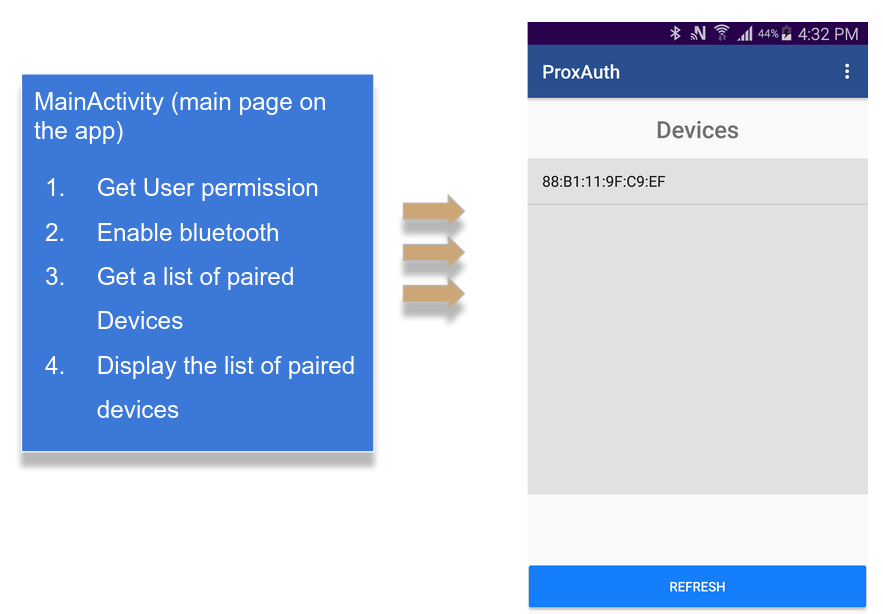
\includegraphics[scale=0.25]{main-activity.png}
\small \textbf{Figure 3: An overview what MainActivity does}
\normalsize

\subsubsection{ControlActivity.kt}
\textbf{ControlActivity} activity is created when the user selects an item (a Bluetooth address) to connect to. \textbf{ContrlActivity} is an activity that spawns a background component called a service that will communicate with the PC the user wishes to communicate with (in our case it is the \textbf{deauth} program running on the user's PC). \textbf{ControlActivity} is a simple activity that will display the alias and the MAC address of the PC the user wishes to connect to. There is also a Disconnect button that will terminate interaction with the PC which will cause \textbf{deauth} to lock the PC.

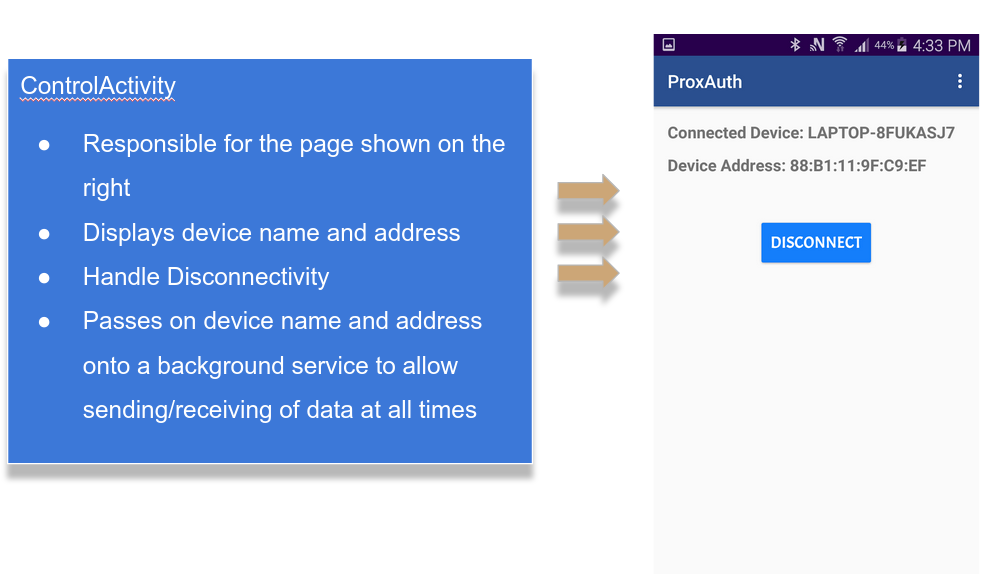
\includegraphics[scale=0.2]{control-activity.png}
\small \textbf{Figure 4: An overview of what ControlActivity does}
\normalsize

\subsubsection{BluetoothInteraction.kt}
\textbf{BluetoothInteraction} is an Android service that runs in the background to facilitate communication with the PC. Once the activity \textbf{ControlActivity} is created, the activity will spawn \textbf{BluetoothInteraction} service and pass on the MAC address of the PC to connect to. The service will attempt to connect with the Bluetooth server running on the user's PC and start sending messages back and forth. Unfortunately, due to time constraints, the current implementation of the application is to continually send "world" to the server and read the string "hello" from the server. The service will just continually communicate with the server until either the server ceases communication or when the user clicks disconnect in \textbf{ControlActivity}. When the user clicks disconnect in \textbf{ControlActivity}, the background service will close communication with the server and terminate. Since a service is a component of the application that runs in the background, it does not interfere with the user's interaction with the phone. The user can put the application out of focus and use their phone for other activities such as checking their email or watching Youtube videos on their phone and it won't interfere with the background service from communicating with the server.

\textbf{Note:} The client (the mobile phone) communicates with \textbf{deauth} using RFCOMM protocol. Refer to \textbf{section 5.4.2} for details on what RFCOMM protocol is or to get an overview of how Bluetooth works.

%%%%%%%%%%%%%%%%%%
%Evaluation and Lessons Learned
%%%%%%%%%%%%%%%%%%
\section{Evaluation and Lessons Learned}
\subsection{Technical and Security Evaluation}

\subsubsection{Technical Evaluation}
Testing is an integral part of our project development cycle. On each iteration, testing on the PAM and de-authentication server has been done to see if the current project satisfies some goals laid out in Section \ref{ssec:num2}. For instance, to test how PAM authenticates users, we have quickly implemented a Bluetooth scanner that will authenticate the user while we work on trying to get the list of paired devices. We figured out testing on a virtual machine does not work very well, so during the development phase, all the testing for de-authentication and PAM was done through Kim's laptop. We used real devices (no virtual machines) to test our application and continually do a regression test to ensure no features implemented from previous sprints broke. Any major features to PAM or de-authentication server were first implemented on small programs to ensure it works as intended before integrating the feature to our project. Some programs created to test our features can be found under \textbf{proxyAuth/bluetooth} and under \textbf{proxyAuth/pam/src/pam\_test.c} but most of the small programs were not pushed to the repository. In addition, any user story and pull requests that Kim has worked on or created were documented in-depth showing how the issue was solved and came with sample test cases that were used to verify that the implementation works (refer to \textbf{Figure 5} to see how a typical documentation written by Kim looks like)\\

To test all the features stated in the design goals for PAM, all Kim needed to do was to see if Kim can authenticate his laptop with his mobile phone. Firstly Kim paired a device that the user does not trust and see if PAM will authenticate it. Once PAM fails to authenticate because the device is not trusted, Kim simply registered the MAC address of the device to indicate the device is trusted and see if the device can now authenticate the laptop now that the device is paired and trusted. In addition, once Kim is able to log onto his laptop using his phone, Kim checked if an instance of the de-authentication server was spawned using the following command: \emph{ps -u zaku | grep deauth}.

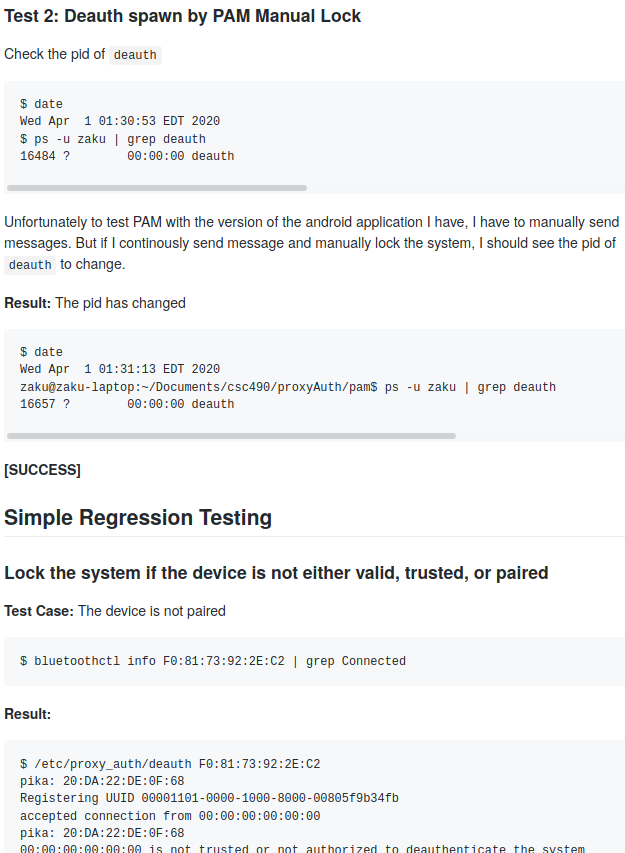
\includegraphics[scale=0.3]{kim_documentation.png}\\
\textbf{Figure 5: A sample how Kim documents and test every issue and pull request assigned to him}

There were many tools and methods used to test the de-authentication server. Firstly, to check whether or not the Bluetooth server is able to communicate with other devices, Daniel and Kim used various Android Applications to simulate a client such as Blueterm to connect to the server and send messages to the server. There was the Android application the team created that was supposed to be able to communicate with the server but when Daniel and Kim initially tested the server and the Android application, it did not work. Therefore to isolate the issue, Kim and Daniel had to use various tools available on the desktop and on the PlayStore to debug where the issues were. But once the issue with communicating with both the Android application and server was resolved, testing was very simple. To test whether or not the server and the android application constantly communicate with each other, we just printed the messages that both the server and client send to each other. To verify whether lock-out works on the de-authentication server, we had the Android device stop sending messages for over 10 seconds and see whether or not the system locks out. To verify proximity check, some modifications to the server was made to print out the bandwidth at each fixed interval and walk out of the room till the system was locked. By observing the changes in bandwidth speed over certain distances, we confirmed the auto-lockout feature works when the user is away from their system.

\subsubsection{Security Evaluation}
Due to time constraints and difficulty getting the Ubertooth One to work the way we want it, there were no security evaluations conducted in the project. The goal of the project was to create a convenient, cheap and secured alternative to password authentication. To test our application's security, the team initially wanted to test a repeater attack and Bluetooth spoofing to see whether or not there were vulnerabilities to the project. However, the team was unsuccessful in having the Ubertooth One to repeat packets and was unable to learn how to spoof Bluetooth MAC addresses on time for the final sprint. Since the team was unable to sniff Bluetooth packets, the team decided to try implementing an encryption scheme to further secure the communication between the authenticator and the PC. The encryption scheme the team tried to implement was AES GCM. AES GCM is known for its high performance while maintaining security[26]. AES GCM is designed to provide both data authenticity, integrity, and confidentiality to allow the user to know whether the data has been tampered or not, the ability to verify the originator of the message and is unreadable by eavesdroppers. However, the team failed to implement any additional layer of encryption on top of the encryption Bluetooth uses.

Therefore, the Bluetooth communication between the PC and authenticator solely relies on the security of Bluetooth which remains to be questionable whether or not Bluetooth security is reliable. There are three aspects of security that Bluetooth needs to provide for our project to be secured: confidentiality, integrity, and authorization. Bluetooth must ensure that the messages being sent between the PC and authenticator cannot be tampered nor read by a malicious entity. Furthermore, no unauthorized devices should be communicating with the PC when the de-authentication server issues a challenge to the authenticator. The security that Bluetooth devices offer vary between different versions of Bluetooth the device supports. For instance, Bluetooth versions 4 and 5 uses Elliptic Curve P-256 pairing algorithm and AES-CCM encryption[27]. AES-CCM is designed to provide both authentication and confidentiality. AES-CCM just like AES-GCM is symmetric encryption and is less computationally expensive compared to asymmetric key encryptions. To authenticate the PC, our implementation relies on the security of Bluetooth pairing. The team will be assuming the security of Bluetooth's implementation of Curve P-256 pairing algorithm is secured. Therefore, ProxyAuth will rely on the underlying Bluetooth security for now and will look into ways to make the project more secure in the future.

Aside from concerns about the security of Bluetooth, there were a few security considerations made when developing the de-authentication server. Since the applications were written in C, there were concerns of introducing security vulnerabilities in the application such as buffer overflow, privilege escalation, and memory access issues. For instance, when reading the list of trusted MAC addresses from the file \textbf{/etc/proxy\_auth/\emph{user}}, there may be malicious contents in the file that would cause the program to crash or cause a buffer overflow. It is unlikely for any malicious input to be written to \textbf{/etc/proxy\_auth/\emph{user}} because the file is owned by root and only the system administrator is allowed to write the list of trusted MAC addresses for each user into the file. Each user in the system has their own file located in \textbf{/etc/proxy\_auth/}.
If the system administrator allows each user to write to the list themselves, the file permissions should be set that only the owner (i.e. the user) should be able to write to the file. However, it is not safe to assume the file is safe. Therefore when PAM and de-authentication server reads from the file, each line in the file gets parsed to ensure each line in the file is a valid Bluetooth MAC address. However, the current implementation of the file sanitizer does cause some worry. Upon writing the report, Kim has noticed when the program reads from the file, it uses \textbf{\emph{getline}} to read each line of the file. This is a concern because Kim is unsure if there is a limit to how long a line can be. A better implementation would be to read only \textbf{BT\_MAC\_LEN} bytes at a time from the file to avoid any possible issues with \textbf{\emph{getline}}. When developing PAM and the de-authentication server, Kim ensured the team compiles the code in a strict manner. Warnings are treated as errors and the \textbf{-fsanitize} flag is used to detect any memory leaks during runtime. Kim has put in a lot of effort to close any possible memory leaks but there can still be bugs that compromise the security of the applications. Memory leaks and illegal access to memory can lead PAM and the de-authentication server to crash leading to a lot of security vulnerabilities with the project. If there are issues with memory access in PAM, it could lead the user to be unable to access their machine. Though this can be resolved by pressing \emph{crtl + shift + f3} to log onto their system via terminal console. However, if the de-authentication server crashes, the lockout feature would be disabled. Meaning the user could leave their system unlocked without the user's notice which leads the system to be vulnerable to malicious entities. Another concern raised with the de-authentication server is the fact that the process can be killed by the attacker. If the user takes their attention away from the system such as having a discussion with a coworker in their cubicle and is physically away from their PC but still nearby their system to not have the PC be locked out, an attacker could kill the de-authentication server. This will leave the system vulnerable when the user leaves their cubicle thinking the system would auto-lock when in reality, the lock-out feature was disabled by a malicious attacker. The team will assume this risk to be low since the window of opportunity is small and unlikely. However, there exists a possible vulnerability with PAM that could lead to the risk of this window of opportunity to increase significantly. PAM authenticates assuming Bluetooth pairing process is secure. PAM does not check the proximity of the authenticator before authenticating the system. A proximity check is only offered in the de-authentication server. If a repeater can extend the range of the authenticator's connection with the user's PC, the attacker can quickly kill the de-authentication server before the program can detect the proximity of the authenticator and thereby giving full access of the PC to the attacker.

\subsection{Timeline and Division of Responsibilities}
\subsubsection{Timeline:}
According to the proposal we have submitted, there were 5 milestones to be completed within the 8 weekly sprints. 

For reference, I shall repeat what the first 3 out of 5 milestones were:
\begin{singlespace}
\begin{enumerate}[noitemsep]
\item Custom operable PAM module that is able to log into the system without a password by Bluetooth pairing.

\item Create an Android application with a basic user interface. The user should have the UI option to select their preferred level of security(zero effort, zero-knowledge, multifactor), though they will not be fully implemented at this time. The app should have basic Bluetooth functionality.  

\item PAM module that pairs with Android application.  The devices should be set to pair with a public key infrastructure exchange to encrypt messages between devices. The user should be required to login to the desktop and enter in a code (similar to two-factor authentication) in the app to authorize the pairing as well as using Bluetooth proximity as a means for future desktop authentication.
\end{enumerate}
\end{singlespace}

Over the course of development, many changes to the direction of our project have changed. 
To not have any members idling, we also worked on Milestone 2 concurrently to develop an Android Application that will communicate with any of the systems that were paired to the mobile device via Bluetooth's RFCOMM protocol. By distributing tasks among various members, we ensure no members were idling. The reason why we were able to finish the first two milestones was that we redundantly assigned each issue to various contributors. We allowed contributors to either work as a group or work on their own to complete their assigned user stories. Not all contributors were available at the same time and had different schedules so adding the flexibility for individuals to choose how they want to tackle the issue was beneficial. For instance, the Android team decided to meet up every Wednesday or Thursday to work no their assigned issues together and asked Kim for any help. Since Kim has a lot more experience when it comes to Android App development and with setting up Linux Machines, it helped the group not be too bottlenecked with setting up their work environment (which still ended up as a big bottleneck) and answer any questions they had about PAM and Android in general. Although it did take a considerable amount of time to have each individual contributor be on the same level of preparedness and knowledge in their assigned tasks, it could have been worse. Milestone 1 was completed in a series of steps that were manageable. By breaking the milestone into series of small steps, it was possible to have a working PAM module that will authenticate the user's system based on if the mobile device is paired and is trusted by the system.

However, we never got far into completing the remaining milestones. We were way too ambitious and lack knowledge of how we were to approach encrypting messages with the device. In addition, it would seem we have ordered some tasks onto the wrong milestone. For instance, according to our proposal, locking the user's device if it fails to respond to the challenge response was implemented in Milestone 1. Though our challenge and response were very simple which was that the device needed to send any message back to the server. Furthermore, it does not seem much work has been completed after the $5^{th}$ sprint and onwards. Other priorities from other courses have hindered our progress with the project. This was probably when communication started to break down and when we started to meet less often to work on issues together. With the lack of time and communication, the project was in a bit of disorder. Figuring out how to encrypt messages took over two sprints and in the end, we never got a working implementation of having encrypted messages to be sent back and forth between the computer and the mobile phone. There has been work started for encrypting messages and creating a protocol of how messages should be structured but it was not completed before the final sprint. The milestones that were worked in the final 4 sprints were Milestone 3 and Milestone 4 which can be summarized as such:
\begin{singlespacing}
\begin{itemize}
\item Create a protocol to how the initial set up with the Android device and the Computer
\item Create a challenge response to the Android device that is secured using a well-thought challenge and using encryption to send the message.
\item Implement whether Bluetooth communication has been intruded by analysing the throughput of Bluetooth packets.
\end{itemize}
\end{singlespacing}

With low motivation, busy schedule, and lack of knowledge on how to use the Ubertooth One device to attack our application, none of the tasks in milestone 3 and milestone 4 has been successfully implemented and tested other than checking proximity of the authenticator.

\subsubsection{Division Of Responsibilities:}
Responsibilities were split into 4 main categories:
\begin{itemize}[noitemsep]
\item PAM
\item De-authentication
\item Android Development
\item Security
\end{itemize}

\textbf{Note:} This is by no means an exhaustive list of what each contributor has done. I am solely basing each contributor from what they have written on their sprint logs and basing from my memory of what they have told me what they were working on.\\

\large
\textbf{Contributers:}
\normalsize

\textbf{Arslan Qamar:} Arslan worked on the Android Development and Security. To be more specific in the security category of the project, Arslan was tasked along with Daniel Xin Wang to discover how to attack our implementation using the Ubertooth One. Arslan also worked on the encryption of the Bluetooth messages. His role in the Android Development was to aid the others in their issues, debug, and test the application. In addition, he was tasked to try to get the application to work in the background.

\textbf{Anurag Bist:} Anurag worked on Android Development along with Sean Coutinho and Arslan Qamar. Anurag wrote most of the code for the Android Application to communicate with the Bluetooth Server (the de-authentication server) to relay messages back and forth. Anurag also worked on trying to get the communication to work in the background. In addition, Anurag also added some additional minor features to the application.

\textbf{Sean Coutinho:} Sean Coutinho worked on the Android Development. He worked with Anurag and Arslan on the Android Development. Sean was tasked with getting the Application to recognize whether or not Bluetooth was on or off, retrieve the list of devices connected to the phone. Sean also tried to create a protocol for the messages being sent between the de-authentication server and the application to potentially add more complex features to the server. Sean also worked on trying to get add encryption and decryption working on the Android application as well as try to get communication with the server done in the background.

\textbf{Areeb Siddiqui:} Areeb worked on the security component, the encryption of Bluetooth messages, of the project while also contributing to the de-authentication server as well such as having the de-authentication server to read and write messages to the Android device.

\textbf{Ju Hong Kim:} Kim was the sole developer for the PAM module and also worked on the de-athuentication server component of the project. Kim has successfully written a PAM module that will authenticate the system if the device is paired and is a device that the system trusts. In addition, Kim has written the initial Bluetooth server and fix any bugs with the de-authentication server. Other work that Kim has worked on to the de-athuentication server such as ensuring the device connected to the server is the device that authenticated the system and have the program be killed when the user locks the system. Kim also helped out with the Android Development as well such as fixing bugs with communicating with the Bluetooth C Server (the de-authentication program). In the latter stage of development when PAM  was completed and the de-authentication server was waiting for new features to be implemented such as the encryption and message protocol that the server and Android application were supposed to follow, Kim was restructuring the code to be more modularized and clean along with writing documentation of what each part of the program is supposed to do, and fix any memory leaks that exist both in PAM and in the de-authentication server. Kim also worked on getting the Android Application to successfully send messages back and forth in the background since the Android team was struggling with the issue for a few sprints and fix other minor issues with the Android application.

\textbf{Daniel Xin Wang:} Daniel's main responsibility was working on the security component of the project. More specifically, to investigate the Ubertooth One's capabilities and devise ways to attack and defend our implementation. Some ideas Daniel has proposed were potential attacks by signal repeaters, man in the middle attack, and spoofing Bluetooth MAC addresses. Daniel has implemented a bandwidth test that will measure the speed of the Bluetooth packets being sent by the Android device to determine the distance of the device from the system. Daniel also contributed to the de-authentication server such as have the system to lock when the mobile application fails the challenge request and also explored how to program Bluetooth by creating a C program that would scan all Bluetooth devices within the vicinity.

\subsection{Hardware and Software Obstacles:}
\begin{itemize}[noitemsep]
\item \textbf{Development Environment}: Working on the project required members to work on a Linux machine. The lab machines do not give us sufficient privileges to work on PAM. Most of the team did not have Linux on their laptop so members opted to use a virtual machine. Members had issues getting the virtual machine to set up with ssh installed due to not having done it before. Therefore, only a limited number of members could test both the Android and PAM along with the de-authentication program. This was a big bottleneck during development. We had members spending countless of hours trying to set up the environment rather than spending those times working on user stories. Without an environment to test their work, the group often had to call me to test their code which often was riddled with bugs. Kim often had to stay up late fixing the code they have submitted for testing.

\item \textbf{Getting Linux to read the laptop's built-in Bluetooth adapter:} When members tried to test PAM and the de-authentication server on their own virtual machines, they have encountered problems getting the virtual machines to recognize the built-in Bluetooth adapters. The solution to have the virtual machine get access to Bluetooth was to buy external Bluetooth adapters. However, this was not a good solution because members still encountered issues connecting to the external Bluetooth Adapters. The virtual machines can recognize the external Bluetooth adapters. But the Bluetooth adapters would not pair with the mobile devices easily and the pairing process took a very long time. Therefore members had to once again change how we test the project by dual booting Ubuntu on their personal machines. However, we had one member who still encountered issues in getting their dual-booted machine to pair with their phone. Instead of getting work done, they spent the time trying to debug their set up with no avail. Members were blocked and could not work on the project nor test the project for a long period of time until Kim was available to test their code.

\item Attacking our implementation using Ubertooth One has failed to materialize. Arslan and Daniel have tried for hours trying to get Ubertooth One to repeat Bluetooth packets. Initially, we thought we could put the Ubertooth One in repeater mode and it would repeat all the packets that the device reads. Unfortunately, that is not how it works. According to Daniel and Arslan who have been researching UbertoothOne, the repeater mode on the Ubertooth is solely for testing the range of the Bluetooth which is different from what we had initially thought.  There has been research in using other tools such as Gattacker which is used to hack into cars via Bluetooth.
\end{itemize}

\subsubsection{Recommendations}

For those who wish to continue this project, here are some recommendation specifically to the project implementation:
\begin{singlespacing}
\begin{itemize}
\item Documentation on Programming Bluetooth is very lacking. Anyone wishing to work on Bluetooth for desktop, the only sole documentation you can really rely on is essentially Albert Huang's documentation on Bluetooth Programming or any documentation that expands on Huang's documentation. Huang created his own documentation about Bluetooth Development solely because there was "virtually no documentation whatsoever"[6]. On the flip side, Google has done a great job of providing documentation on programming Bluetooth on Android.

\item Most of the learning how to work with Bluetooth on Linux other than from Huang's documentation on Bluetooth is through reading various open source source code. Even Huang had to learn from reading the source code of many open-source software projects such as Bluez. Oddly enough, there are a lot of great and mature Bluetooth Desktop applications but not a lot of documentation which is also something Huang has noted in his book. When reading Huang's documentation about Bluetooth, it helps to also cross-reference other source code such as the source code for the Bluetooth library itself. It also helps to read on Bluetooth in general to understand what is actually happening at a much deeper level than what Huang covers.

\item Prepare to read a lot of documentation and source code to work with D-Bus. Fortunately, D-Bus has a lot more documentation in comparison to Bluetooth. However, I had a difficult time reading through the documentation and understanding how to work with D-Bus. I mostly cross-referenced the documentation and other open source projects including GNOME and KDE's source code.

\item If you are going to work with Linux and Bluetooth, install Linux on your machine. It is not worth the pain running a virtual machine and buying a Bluetooth adapter to get it working. It is best for all members to have a working environment as early as possible so that all members can contribute and not wait for another member to test their changes.

\item Communication is extremely crucial. Meet up with members in person and discuss what needs to be done and assign tasks to each member. Appointing a member as a scrum leader would help facilitate communication and ensure every member is on track and working.
\end{itemize}
\end{singlespacing}
\label{Section 6.3}

%%%%%%%%%%%%%%%%%%
% Concluding Remarks
%%%%%%%%%%%%%%%%%%
\section{Concluding Remarks}

The purpose of ProxyAuth is to create an alternative way for users to authenticate their system with zero-effort without any need for the user to lock their system when they leave their system unattended. The goal was to create an authentication system that is cheap, convenient and secure compared to other popular alternatives to authentication such as passwords, fingerprint, and Yubikeys.

The team successfully created a zero-effort authentication to their system by authenticating the user based on the fact that the user has their mobile phone act as an authenticator. The authentication works by checking if the device is paired and trusted by the PC and to continuously authenticate the user if the authenticator is within proximity of the PC. The authenticator will run our Android application to continuously respond to the challenge sent by the PC (which is running a de-authentication server) to remain logged in. As soon as the user leaves a few meters from their PC, the PC will be locked to avoid any intruder from accessing the machine. Calculating proximity is done by calculating the throughput of the messages sent by the authenticator. 

However, the project remains incomplete and may be vulnerable to attacks. Due to time constraints and other obstacles, the continuous authentication remains to be non zero-effort authentication. To gain access to the system is zero-effort but the user must manually tap on the Android application to connect to the de-authentication server to gain continuous authentication. In addition, the challenge the PC issues are too simple and could be spoofed.

The impact the project has on the team is profound. Although the project remains incomplete, the team has created a convenient and cheap alternative way to authenticate their system without the hassle of passwords. Passwords are inherently insecure and tedious, especially when company policy dictates that passwords must be changed every four months and must be long and strong. If the project had more time, the team can create an alternative authentication that provides relatively the same level of security as other competitors such as the Yubikey without the hassle of carrying extra hardware and without the extra cost to us the users. The project is also a continuous proximity based authentication which allows us to leave our systems either intentionally or by clumsiness without fear of malicious actors trying to access our system when left unattended. 

\hrulefill\\
\large \textbf{Learning Outcomes}

\normalsize
The project provided the team personal experience what it takes to create a security product and the difficulties of working with an uncoordinated team with varying backgrounds and experiences. This report will not go over the learning outcomes of other members as this would be purely speculation and grossly inaccurate if attempted. The following learning outcome will only apply to the author. To see the learning outcomes of other members, please refer to the team's report on the project.

\noindent\textbf{Teamwork Learning Outcomes:} From my previous experience with working on a project with a large group of students, it is very difficult to coordinate with the team. This project was no different. The lack of communication and the refusal to follow software engineering practice in the team has caused major headaches for every single member in the team.\\

\noindent\textbf{Workflow Learning Outcomes:} When working on the project, it was neat to work on various collaboration tools even if I was the only member who was actively using the tools. Github Issue Board was great to visualize the overall progress of the project. I even adopted using a Kanboard Board to help me visualize my daily tasks. Github offers a lot of neat tools such as Actions to build, test, and deploy code. Github Actions would be great for the team to adopt because I will no longer need to fix or ask members to fix code that they never bothered testing. If configured correctly, the tool should be able to create an APK of the Android application which can then be easily installed to one's phone for testing. Android Studio is a resource hungry application and so I often did not test what the Android team were pushing and just opted to read their code to see what they have done. I also enjoyed Slack's feature to integrate Github to Slack. The feature notifies every member in the channel of any changes to an issue, pull request or if someone has committed some changes to the project. Other tools that would have been interesting to use is creating a template on how each commit, issue, and pull request should be formatted so that I can have members write better commit messages and issues. \\

\noindent\textbf{Linux, Android and C:} Since I like using Linux and programming in C, I like what I have learned from the project. I have learned a lot about Linux such as how Linux authenticates users. Before the project started, I had no clue what PAM was nor knew what GDM was. In addition, I never knew other applications can communicate with each other using D-Bus nor knew how Bluetooth works. The project also taught me a lot about Makefiles, the differences between static and dynamic objects, and how to detect memory leaks by using various instrumentation and profiling tools such as valgrind and \emph{-fsanitize=address}. It was also interesting to learn Kotlin and compare it with Java since I have experience working with Java Android Development.

%%%%%%%%%%%%%%%%%%
% Future Work
%%%%%%%%%%%%%%%%%%
\section{Future Work}

The project has a lot of room for improvements. The project did not even complete its primary design goals. 

\hrulefill

\textbf{Android Application}
\begin{itemize}
\item The list of paired MAC addresses displayed in \textbf{MainActivity} should only display addresses that are configured to be authenticated to the PC. The current list of MAC addresses displayed on the Android application lists MAC addresses that may not even be reachable at the moment. It is meaningless to show any MAC addresses that are not even meant to be connected with the phone for de-authentication purposes such as the MAC addresses of the user's Bluetooth headphones. To approach this issue, there must be a way for users to manually register the MAC addresses by having a new activity that is responsible for registering new address to the application. The new activity can probably list all non-registered Bluetooth devices the user has paired before and have the \textbf{MainActivity} to list only MAC addresses of computers the user wishes to have the device act as an authenticator for. A text file is sufficient enough to store the list of MAC addresses of computers the user wishes to authenticate to as the average user will not have more than two or three computers they authenticate to on a daily basis.

\item Auto pair and communicate with the PC without the user's intervention. Users expect hands-free continuous authentication. Having the user be required to click a single button on their phone each time they log in to get the auto lockout feature does not solve what the project is trying to tackle. Users do not wish and will not remember to manually connect to the de-authentication server because if they did, they would not forget to lock their machines. There has been work on getting this issue resolved but it remains unsolved. The approach to resolving this issue is to have the application to continually try to communicate to the PC the user wishes to connect to in a background service only if the PC is currently paired to the phone.
\item  Add an extra layer of encryption on top of Bluetooth security. The team was unable to get encryption and decryption capabilities on both the Android application and the de-authentication server. The feature is important because it is not safe to assume the underlying technology (Bluetooth) is secure even if Bluetooth has their own encryption scheme.
\item Add extra security options for the user to select. Perhaps the user is uncomfortable having his PC unlocked through Bluetooth pairing only would like to add extra security such as through writing a pin on the application or a button to confirm the request to authenticate. Clicking a button or having the option to authenticate the PC if the Phone is unlocked is much easier than typing a complex password. Most mobile phones have fingerprint readers which are passwordless and convenient forms of authentication. Since most computers do not come with fingerprint scanners, our project could utilize existing fingerprint scanners on the phone to authenticate the user's PC.

\item Create a website where users can report lost or stolen phones to prevent the phone from being used to authenticate their computers. We can have the application to check on our servers if the device is blacklisted from ProxyAuth's server and disable the device if it is blacklisted. This can simply be done by requiring users to create an account with our servers and register the MAC address of their authenticator which would be cryptographically hashed in our database.
\end{itemize}

\hrulefill

\textbf{PAM}
\begin{itemize}
\item Allow customization to PAM to allow multi-factor authentication. There are a few approaches to allow multi-factor authentication working on PAM. The first option is to modify \textbf{gdm-password} PAM configuration file but this requires the user to know how to configure PAM properly and is not flexible to changes. We could create a website that generates a PAM configuration file for \textbf{gdm-password} based on the user's preferences. This is probably the easiest solution to tackle this feature. Another option could be to modularize the team's PAM module to be able to call other PAM modules such as \textbf{pam\_yubico.so} or \textbf{pam\_unix.so} based on the user's preferences.
\item Increase security to PAM by changing how we authenticate users. Currently, we authenticate users based on if the authenticator's MAC address is trusted by the user and is currently paired to the PC. This is relying on the security of Bluetooth pairing process and perhaps should not be trusted. Perhaps we could also require the authenticator to respond to a challenge sent by our PAM module. Furthermore, it may be also in the best interest of security to also add throughput analysis to check the authenticator's proximity from the PC to prevent repeater attacks from getting access to the machine. Proximity check through bandwidth/throughput analysis is currently only supported by the de-authentication server since it would not matter if the attacker can gain access to the machine for a split second and be locked out because it fails proximity check. However, the small frame of opportunity could be used to kill the de-authentication program rendering the auto lock-out feature useless.
\end{itemize}

\hrulefill

\textbf{De-authentication Server}
\begin{itemize}
\item Have the de-authentication server lock the PC if there is no connection from the authenticator within a very small time frame. The current project implementation requires the user to manually connect to the server to start the auto lockout feature. This can easily be done by setting the \textbf{\emph{connect}} function call to non-blocking and if it fails to get a connection from the authenticator in that small time frame, lock the machine.
\item Change how the program locks the PC to add support for other desktop environments such as KDE and Xfce
\item Change D-Bus calls to use \textbf{libdbus} instead of \textbf{GDBus} to support other desktop environments since current implementation support GNOME only.
\item Create a program to customize the user's proximity lockout feature to allow users to customize the distance they wish their PC to be locked.
\item Create a more complex challenge for the server to issue. The current implementation does not care what the authenticator sends as long as it receives a message. Creating a more complex challenge would increase the security of the project and make Bluetooth spoofing and man in the middle attacks much more unlikely to succeed.
\end{itemize}

\hrulefill

\section{References}

{\small
\begin{lstlisting}
[1] Verizon, "2017 Data Breach Investigations Report," (*@\textit{Verizon}@*), 2017. [Online].Available: https://www.ictsecuritymagazine.com/wp-content/uploads/2017-Data-Breach-Investigations-Report.pdf 
    [Accessed March 30, 2020]
\end{lstlisting}
}

{\small
\begin{lstlisting}
[2] S. Palfy, "How Much do Passwords Cost your Business?," (*@\textit{infosecurity}@*), June 14, 2018. 
    [Online], Available: https://www.infosecu
    rity-magazine.com [Accessed March 30, 2020]
\end{lstlisting}
}

{\small
\begin{lstlisting}
[3] HYPR, "New Password Study by HYPR Finds 78% of People Had to Reset a Password They Forgot in Past 90 Days", (*@\textit{HYPR}@*), Dec 10, 2019. [Online], Available: https://www.hypr.com/hypr-password-study-findings/ 
    [Accessed March 29, 2020]
\end{lstlisting}
}

{\small
\begin{lstlisting}
[4] Verizon, "2019 Data Breach Investigations Report," (*@\textit{Verizon}@*), 2019. [Online], Available: https://enterprise.verizon.com/resources/executivebriefs/2019-dbir-executive-brief.pdf [Accessed March 30, 2020]
\end{lstlisting}
}

{\small
\begin{lstlisting}
[5] Microsoft, "Password-less protection: Reduce your risk exposure with password alternatives," (*@\textit{Microsoft}@*), 2018. [Online], Available: https://query.prod.cms.rt.microsoft.com/cms/api/am/binary/RE2KEup [Accessed March 29, 2020]
\end{lstlisting}
}

{\small
\begin{lstlisting}
[6] A. Huang, "An Introduction to Bluetooth Programming: About this booklet," 2008. [Online]. Available: https://people.csail.mit.edu/albert/bluez-intro/ [Accessed Jan. 2020]
\end{lstlisting}
}

{\small
\begin{lstlisting}
[7] J. Bonneau, C. Herley, P. Van. Oorschot and F. Stajano, "The Quest to Replace Passwords: A Framework for Comparative Evaluation of Web Authentication Schemes," 2012 IEEE Symposium on Security and Privacy, San Francisco, CA, 2012, pp. 553-567.
\end{lstlisting}
}

{\small
\lstset{emph={Computer Security and the Internet: Tools and Jewels}, emphstyle=\itshape}
\begin{lstlisting}
[8] Van Oorschot, (*@\textit{"Computer Security and the Internet: Tools and Jewels"}@*),
     Springer, 2019. [E-book]
\end{lstlisting}
}

{\small
\begin{lstlisting}
[9] L. Silver, "Smartphone Ownership Is Growing Rapidly Around the World, but Not Always Equally," (*@\textit{"PEW Research Center"}@*), Feb. 5, 2019. [Online], Available: https://www.pewresearch.org/ [Accessed March 31, 2019]
\end{lstlisting}
}

{\small
\begin{lstlisting}
[10] Statcounter Global Stats, "Mobile Operating System Market Share Worldwide," (*@\textit{Statcounter Global Stats}@*) March 2020. [Online], Available: https://gs.statcounter.com/os-market-share/mobile/worldwide [Accessed April 05, 2020]
\end{lstlisting}
}

{\small
\begin{lstlisting}
[11] A. Merayyan, "Proximity Authentication," (*@\textit{SANS Institute}@*), July 16, 2001. [online document], Available: https://www.sans.org/reading-room/whitepapers/authentication/proximity-authentication-102 [Accessed April 05, 2020]
\end{lstlisting}
}

{\small
\begin{lstlisting}
[12] Ensure Technologies, "XYLOC Solutions Overview," (*@\textit{Ensure Technologies}@*), 2009. [online document], Available: https://www.ensuretech.com/wp-content/uploads/2011/08/xyloc-overview-brochure.pdf [Accessed Apirl 5, 2020]
\end{lstlisting}
}

{\small
\begin{lstlisting}
[13] Apple, "How to unlock your Mac with your Apple Watch," (*@\textit{Apple}@*), Oct. 21, 2019. [Online], Available: https://support.apple.com/en-ca/HT206995 [Accessed 05, 2020]
\end{lstlisting}
}

{\small
\begin{lstlisting}
[14] Apple, "Use Continuity to connect your Mac, iPhone, iPad, iPod touch, and Apple Watch," (*@\textit{Apple}@*), April 31, 2020. [Online], Available: https://support.apple.com/en-ca/HT204681 [Accessed April 5, 2020]
\end{lstlisting}
}

{\small
\begin{lstlisting}
[15] Near Lock, "A new way to lock your Mac. Just walk away.", (*@\textit{Near Lock}@*). [Online], Available: https://nearlock.me/press [Accessed Apirl 05, 2020]
\end{lstlisting}
}

{\small
\begin{lstlisting}
[16] D. Damopoulos, G. Kambourakis, "Hands-Free one-Time and continuous authentication using glass wearable devices," (*@\textit{Journal of Information Security and Applications}@*), vol. 46, p.138-150, June 2019 [Online]. Available: https://arxiv.org/pdf/1810.02496.pdf [Accessed Feb. 2020]
\end{lstlisting}
}

{\small
\begin{lstlisting}
[17] S. Mare, A. M. Markham, C. Cornelius, R. Peterson and D. Kotz, "ZEBRA: Zero-Effort Bilateral Recurring Authentication," (*@\textit{2014 IEEE Symposium on Security and Privacy}@*), San Jose, CA, 2014, pp. 705-720.
\end{lstlisting}
}

{\small
\begin{lstlisting}
[18] K. R, M. JP, C. A, and et al, "Role of computerized physician order entry systems in facilitating medication errors," (*@\textit{JAMA}@*), vol. 293, no. 10,pp. 1197-1203, 2005
\end{lstlisting}
}

{\small
\begin{lstlisting}
[19] A. Morgan, T. Kukuk, "The Linux-PAM Module Writers' Guide," (*@\textit{Linux PAM}@*), Aug. 2010. [Online], Available: http://www.linux-pam.org/Linux-PAM-html/mwg-introduction-description.html [Accessed Feb 2020]
\end{lstlisting}
}

{\small
\begin{lstlisting}
[20] M. Patkar, "5 Common Bluetooth Myths You Can Safely Ignore Now," (*@\textit{Make Use Of}@*), Dec. 25, 2018. [Online], Available: https://www.makeuseof.com/tag/5-myths-bluetooth-can-safely-ignore-now/ [Accessed May 06, 2020]
\end{lstlisting}
}

{\small
\begin{lstlisting}
[21] I. Golatowski, Class Lecture, Topic: "Service DIscovery Protocol (SDP)" Faculty of Computer Science and Eletricial Engineering, University of Rostock, Germany, 2002. [online document], Available: https://www.amd.e-technik.uni-rostock.de/ma/gol/lectures/wirlec/bluetooth_info/sdp.html
\end{lstlisting}
}

{\small
\begin{lstlisting}
[22] Jimblom, "Bluetooth Basics," (*@\textit{Sparkfun}@*), Aug. 26, 2013. [Online], Available: https://learn.sparkfun.com/tutorials/bluetooth-basics/all [Accessed: April 06 2020]
\end{lstlisting}
}

{\small
\begin{lstlisting}
[23] C. Schwingenschlohl, A. Heigl, "Development of a Service Discovery Architecture for the Bluetooth Radio System," (*@\textit{Institute of Communication Networks, Technische Universität München}@*), 2000. [online document], Available: http://dl.ifip.org/db/conf/ifip6-6/eunice2000/paper5-2.pdf
\end{lstlisting}
}

{\small
\begin{lstlisting}
[24] (*@\textit{Bluetooth Specification}@*), Bluetooth Standard 1B, 1999 
\end{lstlisting}
}

{\small
\begin{lstlisting}
[25] A. Huang, L. Rudolph, (*@\textit{Bluetooth Essentials for Programmers}@*). Cambridge:  Cambridge University Press, 2007.
\end{lstlisting}
}

{\small
\begin{lstlisting}
[26] S.Gueron, "AES-GCM for Efficient Authenticated Encryption - Ending the Reign of HMAC-SHA-1?", Standford University, 2013.
\end{lstlisting}
}

{\small
\begin{lstlisting}
[27] Security Boulevard, "What We Need To Know About Bluetooth Security," (*@\textit{Security Boulevard}@*), Nov. 7, 2019. [Online]: Available: https://securityboulevard.com/2019/11/what-we-need-to-know-about-bluetooth-security/ [Accessed April 5, 2020]
\end{lstlisting}
}

{\small
\begin{lstlisting}
[28] Wikipedia, "Bluetooth," (*@\textit{Wikipedia}@*). [Online], Available: https://en.wikipedia.org/wiki/Bluetooth [Accessed April 5, 2020]
\end{lstlisting}
}

{\footnotesize \bibliographystyle{acm}
\bibliography{sample}}

%\theendnotes

%Hands-Free One-Time and ContinuousAuthentication Using Glass Wearable Devices

%PCASA: Proximity based Continuous and SecureAuthentication of Personal Devices

\end{document}







